\documentclass[fleqn]{report}
\usepackage{lineno}
\modulolinenumbers[5]
\addtolength{\textwidth}{1.5cm}

\usepackage{array, booktabs, import, graphicx}  % for midrule etc. in tabular
\usepackage{textcomp}  % for upright \mu
\usepackage[numbers]{natbib}
\usepackage{multicol}
\usepackage{NVU}
\usepackage{glossaries} 
\usepackage{todonotes}
\usepackage{xcolor}
\usepackage[colorlinks]{hyperref}
\AtBeginDocument{
  \hypersetup{
    linkcolor=black,
    citecolor=red,
    urlcolor=blue,
  }
}
\usepackage{glossaryEntries}

\usepackage{amsmath}  % to number equations by section 
\numberwithin{equation}{section}

\usepackage{caption}
\captionsetup{font={small}}

\usepackage{textcomp} % upright textmu
\usepackage[toc,page]{appendix}  % Appendix / Supplementary Material
\usepackage[final]{pdfpages}
%%\documentclass[review,fleqn]{report}
%%
%%\usepackage{lineno}
%%\modulolinenumbers[5]
%%
%%%\journal{Journal of Theoretical Biology}
%%
%%\usepackage{array, booktabs}  % for midrule etc. in tabular
%%\usepackage{textcomp}  % for upright \mu
%%
%%\usepackage{multicol}
%%\usepackage{NVU}
%%\usepackage{glossaries} 
%%
%%\usepackage[colorlinks]{hyperref}
%%\AtBeginDocument{
%%  \hypersetup{
%%    linkcolor=black,
%%    citecolor=black,
%%    urlcolor=black,
%%  }
%%}
%\usepackage{glossaryEntries}

\usepackage{amsmath}  % to number equations by section 
\numberwithin{equation}{section}

\usepackage{caption}
\captionsetup{font={small}}

\usepackage{textcomp} % upright textmu
\usepackage[toc,page]{appendix}  % Appendix / Supplementary Material
\newcommand{\NO}{\text{NO}}
\newcommand{\Na}{\text{Na$^{+}$}}
\newcommand{\Nas}{\text{[Na$^+]_{s}$}}
\newcommand{\Nak}{\text{[Na$^+]_{k}$}}
\newcommand{\eNOSact}{\text{eNOS$_{\text{act}}$}}
\newcommand{\nNOSact}{\text{nNOS$_{\text{act}}$}}
\newcommand{\LArg}{\text{L-Arg}}
\newcommand{\Otwo}{\text{O$_2$}}
\newcommand{\Glu}{\text{Glu}}
\newcommand{\SC}{\text{SC}}
\newcommand{\K}{\text{K$^+$}}
\newcommand{\Ks}{\text{[K$^{+}]_s$}}
\newcommand{\Cl}{\text{Cl$^{-1}$}}
\newcommand{\Cls}{\text{[Cl$^{-1}]_s$}}
\newcommand{\Clk}{\text{[Cl$^{-1}]_k$}}
\newcommand{\HCOs}{\text{[HCO$_{3}^{-1}]_s$}}
\newcommand{\HCOk}{\text{[HCO$_{3}^{-1}]_k$}}
\newcommand{\Kk}{\text{[K$^{+}]_k$}}
\newcommand{\Ca}{\text{Ca$^{2+}$}}
\newcommand{\EET}{\text{EET}}
%\newcommand{\IP3}{\text{[IP$_3]$}}
\newcommand{\EETk}{\text{[EET]$_{k}$}}
\newcommand{\Can}{\text{[Ca$^{2+}]_n$}}
\newcommand{\Cak}{\text{[Ca$^{2+}]_k$}}
\newcommand{\Cai}{\text{[Ca$^{2+}]_i$}}
\newcommand{\Caj}{\text{[Ca$^{2+}]_j$}}
\newcommand{\Cap}{\text{[Ca$^{2+}]_p$}}
\newcommand{\NOn}{\text{[NO]$_n$}}
\newcommand{\NOk}{\text{[NO]$_k$}}
\newcommand{\NOi}{\text{[NO]$_i$}}
\newcommand{\NOj}{\text{[NO]$_j$}}
\newcommand{\On}{\text{[O$_2]_n$}}
\newcommand{\Oa}{\text{[O$_2]_a$}}
\newcommand{\Oi}{\text{[O$_2]_i$}}
\newcommand{\Oj}{\text{[O$_2]_j$}}
\newcommand{\cGMP}{\text{cGMP}}
\newcommand{\microM}{\textmu M} 
\newcommand{\uMpers}{\textmu M\,s$^{-1}$} 
\newcommand{\persec}{s$^{-1}$} 
\newcommand{\umm}{\textmu m} 

\newcommand\e[1]{$\times$10$^{#1}$}
\newcommand{\n}{$^{-1}$}
\newcommand\pNO[1]{\text{$p_{\text{NO},#1}$}} 
\newcommand\cNO[1]{\text{$c_{\text{NO},#1}$}} 
\newcommand\dNO[1]{\text{$d_{\text{NO},#1}$}} 
\newcommand{\RTF}{$\frac{RT}{F}$}

%%%%%%%%%%%%%%%%%%%%%%%
%% Elsevier bibliography styles
%%%%%%%%%%%%%%%%%%%%%%%
%% To change the style, put a % in front of the second line of the current style and
%% remove the % from the second line of the style you would like to use.
%%%%%%%%%%%%%%%%%%%%%%%

%% Numbered
%\bibliographystyle{model1-num-names}

%% Numbered without titles
%\bibliographystyle{model1a-num-names}

%% Harvard
%\bibliographystyle{model2-names.bst}\biboptions{authoryear}

%% Vancouver numbered
%\usepackage{numcompress}\bibliographystyle{model3-num-names}

%% Vancouver name/year
%\usepackage{numcompress}\bibliographystyle{model4-names}\biboptions{authoryear}

%% APA style
%\bibliographystyle{model5-names}\biboptions{authoryear}

%% AMA style
%\usepackage{numcompress}\bibliographystyle{model6-num-names}

%% `Elsevier LaTeX' style
%\bibliographystyle{elsarticle-num}  % %
%%%%%%%%%%%%%%%%%%%%%%%

\bibliographystyle{KathisBibstyle}


\begin{document}

\author{Tim David}
\title{Neurovascular Coupling Equations for Code version 2.0 }
\maketitle
\newpage
\linenumbers
\listoftodos 
%\input{Introduction}  % \include gives new page
%\input{MaterialAndMethods}
%\input{Results}
%\input{Discussion}
%
%%\section*{References}
%\bibliography{mybibfile}
%\newpage
\chapter{Notes for reading}
The following notes, definitions and equations provide the reader with a comprehensive guide to version 1.2 of NVU. The document is set out in sections where each section contains the equations for each compartment, namely neuron, synaptic cleft, astrocyte, perivascular space, smooth muscle cell, endothelial cell, extracellular space and finally the lumen. The reader will find multiple definitions and equations but by dividing the document into sections corresponding to compartments it is hoped that a more clear understanding is obtained.
Concentrations as written on the left-hand-side of the o.d.e. are given by the notation of $N_j$ where j can be any specii such as \Na of \Ca. True concentrations are written with square brackets as in \Can . In point of fact they are equivalent.
%Figure \ref{fig:nvu_FULL} shows a schematic of the ion channels, pumps and pathways.

Subscripts on variable such as concentrations denote the compartment, n=neuron, k=astrocyte, s=synaptic cleft, i=smooth muscle cell, j=endothelial cell, e = extracellular space.  Concentrations with "hats" denote those in the ER/SR stores. 
\subsection{Version 1.2 /2.0 difference}
 The basic difference between version 1.2 and version 2.0 is the new neuron model. This is based on the work of Chang et al \cite{Chang2013}	and that of Kager et al \cite{Kager2000a}. For this version the neuron model has  4 compartments; i) soma/axon, ii) dendrite , iii) post synaptic terminal and extracellular space (ECS). Ion channels for \Na, and \K efflux into the ECS.  \K is buffered in the ECS and a portion of the \K flux is passed into the synaptic cleft compartment. On reaching a certain concentration of \K in the synaptic cleft  glutamate is pumped into the synaptic cleft . This glutamate is taken up by both the post-synaptic neuron and the astrocyte. The neuron is stimulated by injection of a current of specified value into the soma/axon compartment. 
 
 
 In addition Nitric Oxide is derived from the NMDA receptor where glutamate mediates \Ca flux into the post-synaptic neuron. This \Ca is combined with calmodulin to produce eNOS and finally NO.  Schematic of the full set of pathways is shown in Figure \ref{fig:nvu_FULL}
 				 \begin{figure}[h!]
 				\centering
 				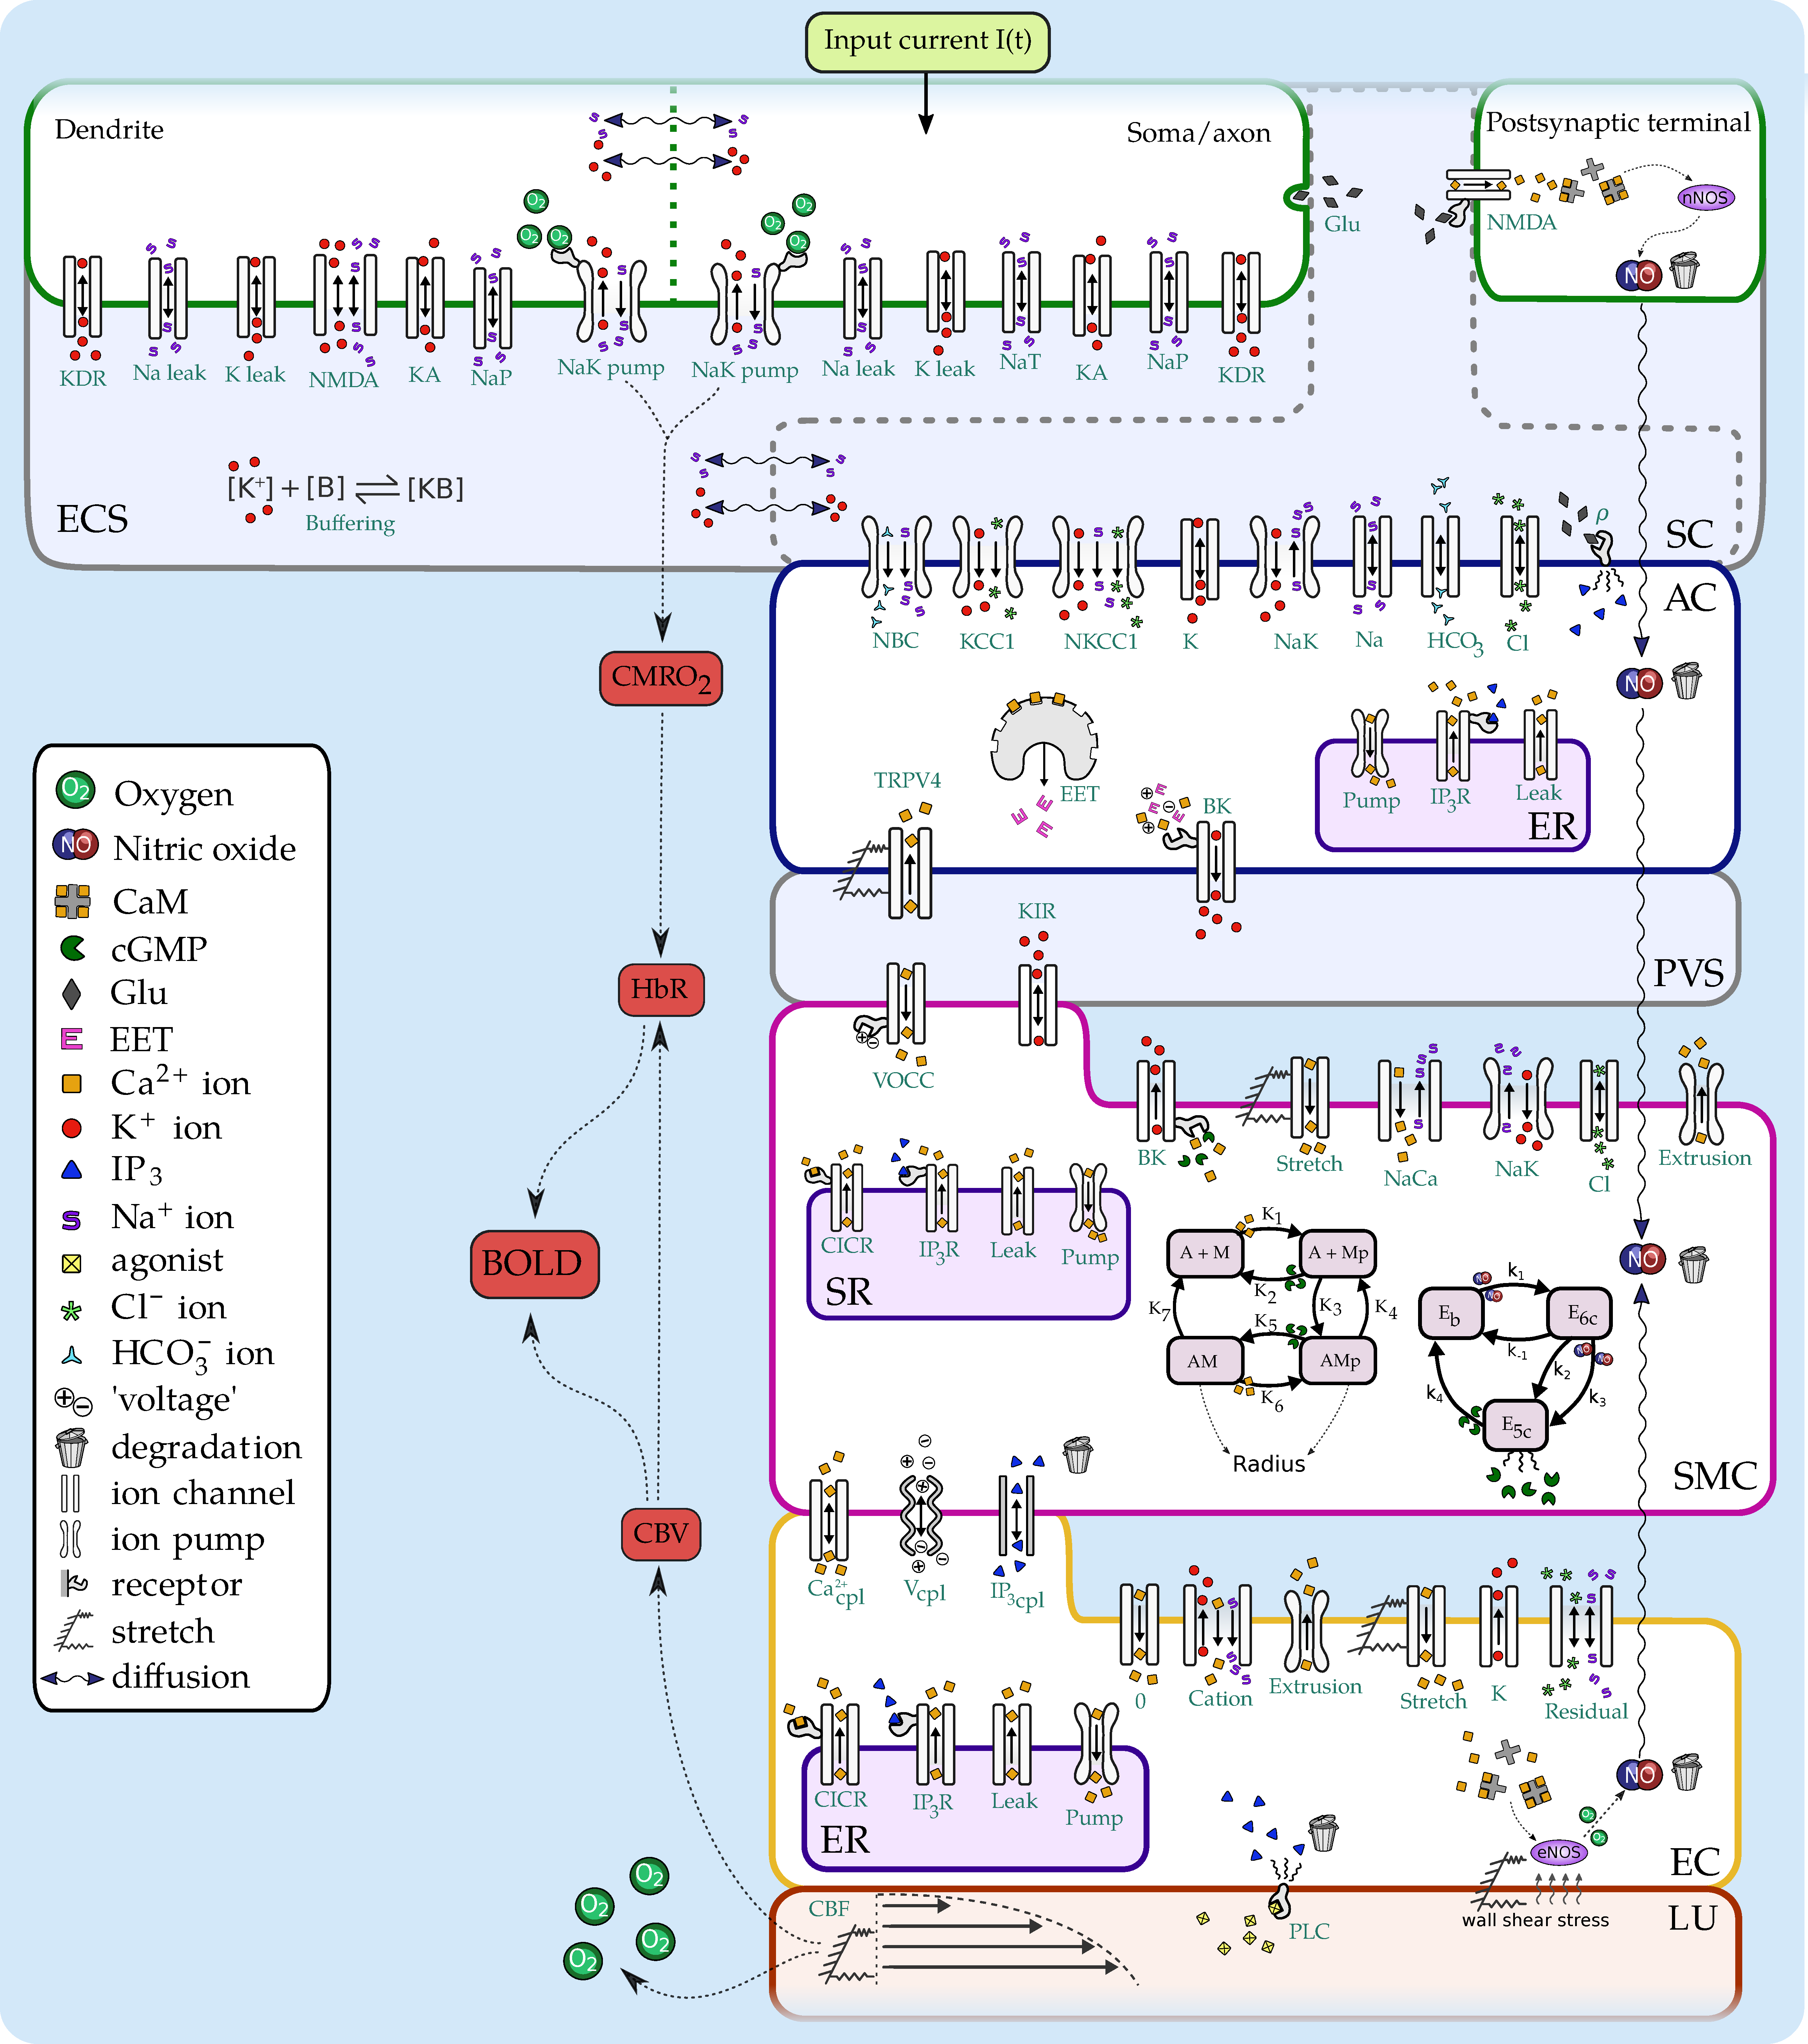
\includegraphics[width=0.8\linewidth]{./nvu_20.pdf}
 				\caption{Schematic of version 1.2}
 				\label{fig:nvu_FULL}
 				\end{figure}


\section{\textbf{Global Constants}}\label{sec:equations}
	\begin{table}[h!]
		\centering
			\begin{tabular}{ p{0.1\linewidth}  >{\footnotesize} p{0.41\linewidth}  >{\footnotesize} p{0.20\linewidth} >{\footnotesize} p{0.27\linewidth} }
			\hline
			$ F $				& Faraday's constant 	& 96500 C mole$^{-1}$ & 	\\
			$ T $				& Temperature				& 300 K				 		&	\\
			$ R_{gas} $	  & Gas constant				& 8.315 J mole K$^{-1}$ &  	\\

			\hline
		\end{tabular}
	\end{table}
	
%	For version 1.2 there are essentially three fluxes from the pre-synapse entering the synaptic cleft, 1) \K, 2) \Na , and \Glu (glutamate). 

				\subsection{The Neuron Model}
%				The neuron model is based on the work of Chang et al\citep{Chang2013} who studied the effects of hypoxic conditions on cortical spreading depression and used to describe neural activation, restoration of ionic gradients and consumption of Na${^+}$/K${^+}$ -ATPase pump. The three major ions sodium, potassium and chlorine and their associated ion channels which contribute to the neural activation are considered in their model. There are three compartments namely soma, dendrite and extracellular space.
				\subsubsection{Ion channels,Cross membrane currents and the Na${^+}$/K${^+}$ exchange pump} 
				The soma compartment has two sodium ion channels namely the persistent sodium and sodium leak channels and three potassium channels namely delayed rectifier potassium channel, transient potassium channel and potassium leak channel . In addition to these the dendrite compartment also has an N-methyl-D-aspartate(NMDA) receptor mediated channel which can allow both the sodium and potassium currents to flow through it. The cross-membrane currents of all the ion channels except the leak ion channel were modelled using the Goldman-Hodgkin-Katz(GHK) equation given as
				 \begin{equation} %\label{eq:Math_appr1}\\
				 \begin{aligned}
				I_{Ion,GHK}=m^{p}h^{q}\frac{g_{Ion,GHK}Fv_m[[Ion]_i-exp(\frac{-v_m}{\phi})[Ion]_e]}{\phi[1-exp(\frac{-v_m}{\phi})]}\\
				\end{aligned}
				\end{equation} 
				where $I_{Ion,GHK}$ is the current of a particular ion through an ion channel, $ g_{Ion,GHK} $ is the maximal conductance value and permeability is absorbed into this parameter, $v_m$ is the membrane potential, $\phi=PT/F$ where $P$ is the universal gas constant , $T$ the absolute temperature and $F$ Faraday's constant, $[Ion]_i$  and $[Ion]_e$ are the concentrations of a particular ion inside and outside the membrane respectively. The conductance is channel specific and concentration of ion is compartment specific. The electrically excitable property of the neuron is simulated using the classical Hodgkin Huxley kinetic description \citep{Hodgkin1952}. The variables $m$ and $h$ are the fraction of activation and inactivation gates in the open state respectively. The parameters $p$ and $q$ are the number of individual activation and inactivation gates per channel respectively. The rate at which the activation gates open and close in response to the membrane potential is modelled according to the equation
				\begin{equation} %\label{eq:Math_appr1}
				\dfrac{\mathrm{d}m}{\mathrm{d}t}=\frac{m_{\infty}(v_m)-m}{\tau_m(v_m)}
				\end{equation}
				where 
				\begin{equation} %\label{eq:Math_appr1}
				m_{\infty}(v_m)=\frac{\alpha_m(v_m)}{\alpha_m(v_m)+\beta_m(v_m)}
				\end{equation}
				and
				\begin{equation} %\label{eq:Math_appr1}
				\tau_m(v_m)=\frac{1}{\alpha_m(v_m)+\beta_m(v_m)}
				\end{equation}
				The function $m_\infty(v_m)$ is called the steady-state activation curve. The value of $m$ tends asymptotically to the steady state if voltage is held constant for a sufficient length of time. The function $\tau_m$ is the characteristic time curve of the activation gate describing the variation of the characteristic time scale with of the membrane potential. 
				%These equations state that the closed activation gates, $(1-m)$, open at rate $\alpha_m(v_m)$, while the open activation gates, $m$, close at a rate $\beta_m(v_m)$. The rate functions, $\alpha_m(v_m)$ and $\beta_m(v_m)$, are functions that depend on the voltage across the membrane. Similarly the rate at which the inactivation gates close in response to membrane potential is modeled. Thus the varying response of different channels to membrane potential is modeled with the experimental data containing maximal conductance and rate functions of the activation and inactivation gates of the individual channels. 
				The rate functions $\alpha$ and $\beta$ are usually determined through a mix of theoretical and empirical considerations and they are of the form
				\begin{equation} %\label{eq:Math_appr1}
				\alpha(v_m)=a_0 \exp(\frac{-\delta{v_m}}{s})
				\end{equation}
				\begin{equation} %\label{eq:Math_appr1}
				\beta(v_m)=b_0 \exp(\frac{(1-\delta){v_m}}{s})
				\end{equation}
				where $ a_0 $, $ b_0 $, and $ \delta $ are positive constants, with $0 \leq\delta\leq 1 $. A gate that tends to open on depolarization will have $s < 0$, while a gate that tends to open on hyperpolarisation will have $s > 0$ \citep{Willms1999}. These exponential forms are modified to fit the experimental data using curve fitting. The expressions used in the neuron model that describe the voltage-dependent rate functions are based on a model of hippocamppal pyramidal cells \citep{Traub1994} and morphological parameters are based on reconstructed hippocampal neurons \citep{Cannon1998}. The sodium, potassium and chlorine leak currents are calculated by a Hodgkin-Huxley(HH) model given by
				 \begin{equation} %\label{eq:Math_appr1}
				I_{Ion,HH}=g_{Ion,HH}(v_m-E_{Ion})
				\end{equation} 
				where $g_{Ion,HH}$ is the constant conductance for the specific ion and $E_{Ion}$ is the Nernst potential for the specific ion and is given by 
				\begin{equation} %\label{eq:Math_appr1}
				E_{Ion}=\frac{PT}{zF}log\frac{[Ion]_e}{[Ion]_i}
				\end{equation}
				here $z$ is the valence of the ionic species. The primary role of the Na${^+}$/K${^+}$ ATPase exchange pump in the neuronal membrane is to restore ionic concentrations to their homeostatic state during neural activation. The Na${^+}$/K${^+}$ ATPase pump is a transmembrane protein with two extracellular binding sites for potassium, three intracellular binding sites for sodium, and a single intracellular binding site for ATP.  The pump moves out three intracellular sodium ions and two extracellular potassium ions against their electrochemical gradients and hence the need for ATP (energy). Both the soma and dendrite compartments have a Na${^+}$/K${^+}$ exchange pump. Since the energy in the form of ATP is highly dependent on tissue oxygen concentration, the exchange pump current in the neuronal membrane is modelled as a variable dependent on the availability of oxygen. The potassium and sodium pump currents in the soma and dendrite are given by $I_{*,K,pump}=-2I_{*,pump}$ and $I_{*,Na,pump}=3I_{*,pump}$ respectively($*$ is either s for somatic or d for dendritic). The total current due to the sodium/potassium exchange pump in the soma and dendrite is given by
				\begin{equation} %\label{eq:Math_appr1}
				\begin{aligned}
				I_{*,pump}=I_{max}\gamma_{*,pump,1}([K^+]_e,[Na^+]_i,*)\gamma_{*,pump,2}([O_2])\\
				\end{aligned}
				\end{equation}
				where $I_{max}$ is the maximum pumping rate of the Na${^+}$/K${^+}$ exchange pump with
				\begin{equation} \label{eq:Math_pump1}
				\begin{aligned}
				\gamma_{*,pump,1}([K^+]_e,[Na^+]_i,*)=\left(1+\frac{[K^+]_{e,0}}{[K^+]_e}\right)^{-2}\left(1+\frac{[Na^+]_{i,0}}{[Na^+]_{i,*}}\right)^{-3}\\
				\end{aligned}
				\end{equation}
				where $[K^+]_{e,0}$ and $[Na^+]_{i,0}$ are the baseline concentrations of extracellular potassium and intracellular sodium respectively. This expression describes that the action of the pump depends on the concentrations of extracellular potassium and intracellular sodium. The second pump represents the oxygen dependent production of ATP by the mitochondria\citep{Cloutier2009,Heinrich1996} taking the form
				\begin{equation} \label{eq:Math_pump2}
				\gamma_{*,pump,2}([O_2])=2\left(1+\frac{[O_2]_0}{(1-G)[O_2]+G[O_2]_0}\right)^{-1}
				\end{equation}
				in this case $[O_2]$ is the tissue oxygen concentration encompassing the neurovascular unit, $[O_2]_0$ is the initial equilibrium value of oxygen concentration and $G$ is the percentage of ATP production that is independent of oxygen. This expression indicates that the pumping rate will be reduced whenever there is a decrease in the oxygen level in the tissue.
				
				
				
				\subsubsection{Membrane potential and Ionic concentration}
				In reality the membrane potential depends on the membrane potential difference and concentration gradients. Here, the membrane potential of the soma and dendrite is calculated based on the assumption that the flow of ions between the two compartments is only due to the difference in membrane potential between them. The total cross membrane currents are the sum of the voltage dependent sodium and potassium currents, sodium, potassium and chlorine leak currents, and the sodium-potassium exchange current. The membrane potentials of the neuronal compartments are governed by the differential equations of the form
				\begin{equation} %\label{eq:Math_appr1}
				C_{m}\dfrac{\mathrm{d} v_{m,s}}{\mathrm{d} t} = -I_{s,tot}+\frac{1}{2R_a\delta_d^{2}}(v_{m,d}-v_{m,s})+I_{stim}
				\end{equation}
				\begin{equation} %\label{eq:Math_appr1}
				C_{m}\dfrac{\mathrm{d} v_{m,d}}{\mathrm{d} t} = -I_{d,tot}+\frac{1}{2R_a\delta_d^{2}}(v_{m,s}-v_{m,d})
				\end{equation}
				here $C_m$ is the membrane capacitance per unit surface area, $R_a$ is the input resistance of the effective dendritic tree, $\delta_d$ is the half length of the effective dendritic tree,$v_{m,s}$ and $v_{m,d}$ are the membrane potentials of soma and dendrite respectively. $I_{stim}$ is the stimulating current in Gaussian form whose mean, variance and amplitude can be allowed to vary. $I_{s,tot}$ and $I_{s,tot}$ are the total cross-membrane ionic currents per unit surface area for soma and dendrite written as
				 \begin{equation} %\label{eq:Math_appr1}
				I_{*,tot}=I_{*,Na,tot}+I_{*,K,tot}+I_{*,Cl,tot}
				%\end{equation}
				% \begin{equation} %\label{eq:Math_appr1}
				%I_{d,tot}=I_{d,Na,tot}+I_{d,K,tot}+I_{d,Cl,tot}
				\end{equation}
				%$I_{s,Na,tot}$, $I_{s,K,tot}$, $I_{s,Cl,tot}$ are the total ionic currents of sodium ,potassium and chlorine ions of the soma respectively and $I_{d,Na,tot}$, $I_{d,K,tot}$, $I_{d,Cl,tot}$ are the total ionic currents of sodium ,potassium and chlorine ions of the dendrite respectively.
				The rates of change of ionic concentration in the soma and dendrite are due to the membrane currents and the exchange between the soma and dendrite. The exchange between the somatic and dendritic compartments is modelled by a flux proportional to the difference between their ion concentrations. The equation describing the rate of change of ions in the soma is again of the general form
				\begin{equation} %\label{eq:Math_appr1}
				\begin{aligned}
				\dfrac{\mathrm{d} [Ion]_{i,s}}{\mathrm{d} t} = -\frac{A_s}{FV_s}I_{s,Ion,tot}+\frac{D_{Ion}(V_d+V_s)}{2\delta_d^2V_s}([Ion]_{i,d}-[Ion]_{i,s})\\
				\end{aligned}
				\end{equation}
				The notation, $ D_{Ion} $ , is the ion diffusion coefficient in aqueous solution taking into account tortuosity and volume fraction \citep{Nicholson1981}. The quantities $A_s  $ and $ A_d $ are the surface areas of the soma and dendrite respectively in the total fixed volume given by the sum of the fixed somatic volume $ V_s $, dendritic volume$ V_d $, and extracellular volume,$ V_e $. The equation describing the rate of change of ions in the dendrite is  
				\begin{equation} %\label{eq:Math_appr1}
				\begin{aligned}
				\dfrac{\mathrm{d} [Ion]_{i,d}}{\mathrm{d} t} = -\frac{A_d}{FV_d}I_{d,Ion,tot}+\frac{D_{Ion}(V_s+V_d)}{2\delta_d^2V_d}([Ion]_{i,s}-[Ion]_{i,d})\\
				\end{aligned}
				\end{equation}
				The local rates of change of the extracellular space ions are due to the membrane currents from the soma and dendrite.  To ensure electro-neutrality, the initial extracellular concentration of the anion $ Cl^- $ is chosen to be equal to the sum of the concentration of cations $Na^+ $ and $K^+ $ in the extracellular space. Also, the initial intracellular concentration of chlorine is chosen in such a way that its Nernst potential matches a resting membrane potential of -70 mV. The existence of immobile anions has been assumed in the soma and dendrites to achieve intracellular electro-neutrality.The equations describing the rate of change of ions in the extracellular compartment is given by
				\begin{equation} %\label{eq:Math_appr1}
				\dfrac{\mathrm{d} [Ion]_{e}}{\mathrm{d} t} = \frac{1}{f_eF}\left(\frac{A_sI_{s,Ion,tot}}{V_s}+\frac{A_dI_{d,Ion,tot}
				}{V_d}\right)
				\end{equation}
				where extracellular space volume fraction is given by $ f_e={V_e}$/${(V_s+V_d)} $. The extracellular space volume was defined as 15\% of the intracellular  space volume based on published data \citep{Mazel1998,McBain1990}.
				
			
				\chapter{State variables, initial values and parameter values}
				In the actual Matlab code the state variables are defined as follows 
				%% State variables
				            
				            % Elshin neuron model
				            $v_{sa}$      : membrane potential of soma/axon, mV
				            $v_d$        :membrane potential of dendrite, mV
				            $K_{sa}$      : K+ concentration of soma/axon, mM
				            $K_d$ :  K+ concentration of dendrite, mM
				            $Na_d$ :  Na+ concentration of dendrite, mM
				            $K_e$ : K+ concentration of ECS, mM
				            $Na_e$ :Na+ concentration of ECS, mM
				            $Buff_e$ : Buffer concentration for K+ buffering in ECS, mM
				 
				          
				            
				             \textbf{Gating variables}
				            m1 : Activation gating variable, soma/axon NaP channel (Na+)
				            m2 : Activation gating variable, soma/axon KDR channel (K+)
				            m3 : Activation gating variable, soma/axon KA channel (K+)
				            m4 : Activation gating variable, dendrite NaP channel (Na+)
				            m5 : Activation gating variable, dendrite NMDA channel (Na+)
				            m6 : Activation gating variable, dendrite KDR channel (K+)
				            m7 : Activation gating variable, dendrite KA channel (K+)
				            m8 : Activation gating variable, soma/axon NaT channel (Na+)
				            
				            h1 : Inactivation gating variable, soma/axon NaP channel (Na+)
				            h2 : Inactivation gating variable, soma/axon KA channel (K+)
				            h3 : Inactivation gating variable, dendrite NaP channel (Na+)
				            h4 : Inactivation gating variable, dendrite NMDA channel (Na+)
				            h5 : Inactivation gating variable, dendrite KA channel (K+)
				            h6 : Inactivation gating variable, soma/axon NaT channel (Na+)
				            
				            \textbf{NO pathway} 
				            $Ca_n$ :\Ca in the post-synaptic neuron                  
				            $nNOS_act_n$ :activated NOS in the post-synaptic neuron
				            $NO_n$ : Nitric Oxide in the post-synaptic neuron
				            
				            	\begin{table*}[h!]
				            				\centering
				            				\caption{Initial resting values and other parameter values of the neuron model, from Chang et al\citep{Chang2013}}
				            				\begin{tabular}{| p{0.15\linewidth} | >{\footnotesize} p{0.14\linewidth} | >{\footnotesize} p{0.14\linewidth} | >{\footnotesize} p{0.4\linewidth} |}
				            				\hline
				            				
				            				\bf Parameters		& \bf Values  & \bf Units  &\bf Description      \\
				            				
				            				\hline
				            				$v_m$&$-70$&$mV$&membrane petential\\
				            				$[K^+]_e$&$3.5$&$mM$&extracellular space potassium ion concentration\\
				            				$[K^+]_i$&$133.5$&$mM$&intracellular potassium ion concentration of neuron\\
				            				$[Na^+]_e$&$140$&$mM$&extracellular space sodium ion concentration\\
				            				$[Na^+]_i$&$10$&$mM$&intracellular sodium ion concentration of neuron\\
				            				$[O_2]_0$&$2\times10^{-2}$&$mM$&baseline concentration of oxygen in the tissue\\
				            				$B_{0}$&$0.9$&$ml$/$100mg$/$s$&baseline cerebral blood flow\\
				            				$[O_2]_b$&$4\times10^{-2}$&$mM$&blood oxygen concentration\\
				            				$J_0$&$2.5\times10^{-2}$&$mM$/$s$&steady state change in oxygen concentration due to cerebral blood flow \\
				            				$R_a$&$1.83\times10^5$&$\Omega$&input resistance of dendritic tree\\
				            				$\delta_d$&$4.5\times10^{-2}$&$cm$&half-length of dendrite\\
				            				$A_s$&$1.586\times10^{-5}$&$cm^2$&surface area of soma\\
				            				$A_d$&$2.6732\times10^{-4}$&$cm^2$&surface area of dendrite\\
				            				$V_s$&$2.160\times10^{-9}$&$cm^3$&volume of soma\\
				            				$V_d$&$5.614\times10^{-9}$&$cm^3$&volume of dendrite\\
				            				$S_e$&$4.1179\times10^{-6}$&$cm$&volume to surface area ratio of the extracellular space\\
				            				$C_m$&$7.5\times10^{-5}$&$s$/$\Omega cm^2$&membrane capacitance\\
				            				$I_{max}$&$1.48\times10^{-3}$&$mA$/$cm^2$&$Na^+/K^+-$ATPase rate\\
				            				$D_{Na^+}$&$1.33\times10^{-5}$&$cm^2/s$&Sodium diffusion coefficient\\
				            				$D_{K^+}$&$1.96\times10^{-5}$&$cm^2/s$&Potassium diffusion coefficient\\
				            				$D_{Cl^-}$&$2.03\times10^{-5}$&$cm^2/s$&Chlorine diffusion coefficient\\
				            				 
				            				\hline
				            				
				            				\end{tabular}
				            				\end{table*}
				            				
				            \begin{table*}[h!]
				            				\centering
				            				\caption{Rate expressions and parameter values used in the voltage dependent channel currents of the neuron model, from Chang et al\citep{Chang2013}}
				            				\begin{tabular}{| p{0.15\linewidth} | >{\footnotesize} p{0.1\linewidth} | >{\footnotesize} p{0.1\linewidth} | >{\footnotesize} p{0.4\linewidth} |}
				            				\hline
				            				
				            				\bf Currents 		& \bf $g_{Ion,GHK} $  & \bf Gates     & \bf Voltage dependent rate functions  \\
				            				$mA/cm^2$&$ mA cm $&$m^ph^q$& \\
				            				\hline
				            				
				            				$I_{Na,P}$			& $2\times10^{-6}$ & $m^2h$ & $\alpha_m=\frac{1}{6(1+exp[-(0.143E_m+5.67)])}$  \\ 
				            				&&& $\beta_m=\frac{exp[-(0.143E_m+5.67)]}{6(1+exp[-(0.143E_m+5.67)])}$\\
				            				
				            				&&& $\alpha_h=5.12\times10^{-8}exp[-(0.056E_m+2.94)] $\\
				            				
				            				&&& $\beta_h=\frac{1.6\times10^{-6}}{1+exp[-(0.2E_m+1.25)]}$\\
				            				
				            				\hline
				            				$I_{K,DR}$			& $10\times10^{-5}$ & $m^2$ & $\alpha_m=0.016\frac{E_m+34.9}{1-exp[-(0.2E_m+6.98)]}$  \\ 
				            				&&& $\beta_m=0.25exp[-(0.25E_m+1.25)]$  \\
				            				\hline
				            				$I_{K,A}$			& $1\times10^{-5}$ & $m^2h$ & $\alpha_m=0.02\frac{E_m+56.9}{1-exp[-(0.1E_m+5.69)]}$  \\ 
				            				&&& $\beta_m=0.0175\frac{E_m+29.9}{exp(0.1E_m+2.99)-1}$\\
				            				&&& $\alpha_h=0.016exp[-(0.056E_m+4.61)] $\\
				            				&&& $\beta_h=\frac{0.5}{1+exp[-(0.2E_m+11.98)]}$\\
				            				\hline
				            				$I_{NMDA}$			& $1\times10^{-5}$ & $mh$ & $\alpha_m=\frac{0.5}{1+exp\left(\frac{13.5-[K^+]}{1.42}\right)}$  \\ 
				            				&&& $\beta_m=0.5-\alpha_m$\\
				            				&&& $ \alpha_h=\frac{1}{2000\left(1+exp\left[\frac{[K^+]_e-6.75}{0.71}\right]\right)} $\\
				            				&&& $\beta_h=5\times10^{-5}-\alpha_h$\\
				            				\hline
				            				\end{tabular}
				            				\end{table*}
				
				            
	\chapter{Equations for each  compartment }
	\section{Neuron}
	\subsection{Nernst potential for Na,K ions in soma and dendrite (Cl constant)} 
				            				\begin{eqnarray}
				            %				E_Na_{sa}     = \RTF  log(Na_e ./ Na_{sa}); \\
				            %								            E_K_{sa}      = \RTF  log(K_e ./ K_{sa});\\
				            %								            E_Na_d      = \RTF  log(Na_e ./ Na_d);\\
				            %								            E_K_d       = \RTF  log(K_e ./ K_d);
				            					E_{Na_{sa}}=\frac{RT}{F}ln (\frac{Na_e}{Na_{sa}}) \\
				            					 E_{K_{sa}}      =\frac{RT}{F}  ln(\frac{K_e}{K_{sa}})\\
				            					 E_{Na_{d}}      =\frac{RT}{F}  ln(\frac{Na_e}{Na_{d}})\\
				            					 E_{K_{d}}      =\frac{RT}{F}  ln(\frac{K_e}{K_{d}})
				            				\end{eqnarray}
	\subsection{Leak fluxes of Na,K,Cl in soma and dendrite using HH}
				 \begin{eqnarray}
				J_{Naleak_{sa}} &=& g_{Naleak_{sa}} (v_{sa} - E_{Na_{sa}})\\
								                        J_{Kleak_{sa}}  &=& g_{Kleak_{sa}} (v_{sa} - E_{K_{sa}})\\
								                        J_{Naleak_{d}}  &=& g_{Naleak_d} (v_d - E_{Na_{d}})\\
								                        J_{Kleak_{d}}   &=& g_{Kleak_d} (v_d - E_{K_{d}})\\
				 \end{eqnarray}
				                        
	\subsection{Dendrite (with subscript d)}
	 \textbf{Na flux through NaP channel in dendrite using GHK}\\
	 
	\begin{eqnarray}
		            m4_{\alpha}    & = &\frac{1}{6  (1 + exp(-((0.143  v_d) + 5.67)))} \\
	                m4_{\beta}     &=& \frac{exp(-((0.143 v_d) + 5.67))}{6  (1 + exp(-((0.143  v_d) + 5.67)))}\\ 
	            h3{\alpha}     &=& 5.12e-8  exp(-((0.056  v_d) + 2.94))\\
	            h3{\beta}      &=& \frac{1.6e-6}{1 + exp(-(((0.2 * v_d)) + 8))}\\
	            J_{NaP_{d}}     &=& (m4^2  h3  g_{NaP} F v_d \frac{(Na_d - (exp(\frac{-v_d F}{RT})  Na_e)))}{(\frac{RT}{F} (1 - exp(\frac{-v_d F}{RT})))} \\
	\end{eqnarray}

	
 \textbf{Na/K flux through NMDA channel in dendrite using GHK}
 \begin{eqnarray}
	            m5_{\alpha}     &=& \frac{0.5}{1 + exp(\frac{13.5 - K_e}{1.42})}\\
	            m5_{\beta}      &=& 0.5 - m5_{\alpha}\\
	            h4_{\alpha}     &=& \frac{1}{2000 * (1 + exp(\frac{K_e - 6.75}{0.71}))}\\
	            h4_{\beta}      &=& 5 \times 10^{-4} - h4_{\alpha}\\
	            J_{NMDA_{K_d}}   & =& M(v,Mg)( (m5  h4  g_{NMDA} F v_d  \frac{(K_d - (exp(\frac{v_d F}{RT})  K_e)))}{(\frac{RT}{F} (1 - exp(\frac{-v_d F}{RT})))}\\
	            M(v,Mg)&=& \frac{1}{(1 + 0.33Mg  \quad exp(-(0.07  v_d + 0.7)))}
 \end{eqnarray}

%	
%	            
 \textbf{K flux through KDR channel in dendrite using GHK}
 \begin{eqnarray}
	            m6_{\alpha}     &=&\frac{0.016  ((v_d + 34.9)}{(1 - exp(-((0.2 * v_d) + 6.98))))}\\
	            m6_{\beta}      &=&  0.25 exp(-((0.025 * v_d) + 1.25))\\
	           J_{KDR_{d}}    & =& m6^2  g_{KDR} F v_d \frac{(K_d - (exp(\frac{-v_d F}{RT})  K_e))}{(\frac{RT}{F} (1 - \frac{-v_d F}{RT}))}
 \end{eqnarray}

%	
\textbf{ K flux through KA channel in dendrite using GHK}
\begin{eqnarray}
	            m7_{\alpha}     &=& \frac{0.02  ((v_d + 56.9)}{(1 - exp(-((0.1  v_d) + 5.69))))}\\
	            m7_{\beta}      &=&  \frac{0.0175  ((v_d + 29.9)}{(exp(((0.1 * v_d) + 2.99)) - 1))}\\
	            h5_{\alpha}     &=& 0.016  exp(-((0.056 v_d) + 4.61))\\
	            h5_{\beta}      &=&\frac{0.5}{(1 + exp(-((0.2 * v_d) + 11.98)))}\\
	            J_{KA_{d}}     & =& m7^2  h5 g_{KA} F v_d  \frac{(K_d - (exp(\frac{-v_d F}{RT})  K_e))}{(\frac{RT}{F} (1 - \frac{-v_d F}{RT}))}
\end{eqnarray}	
\subsection{Soma/Axon (with subscript sa)}			
\textbf{Na flux through NaP channel in soma using GHK}
\begin{eqnarray}
	            m1_{\alpha}     &=& \frac{1}{6 (1 + exp(-(0.143  v_{sa} + 5.67)))}\\ % 0.143 parameter has skewed distribution to the upper end of the uniform pdf, with respect to a flat K_e profile 
	            m1_{\beta}     & =& \frac{exp(-0.143  v_{sa} + 5.67)}{ 6 (1 + exp(-(0.143  v_{sa} + 5.67)))}\\
	            h1_{\alpha}     &=&  5.12 \times 10^{-8} exp(-(0.056  v_{sa} + 2.94))\\
	            h1_{\beta}      &=& \frac{1.6 \times 10^{-6}}{1 + exp(-(0.2  v_{sa} + 8))}\\
	            J_{NaP_{sa}}    &=& m1^2  h1 g_{NaP} F v_{sa}  \frac{(Na_{sa} - (exp(\frac{-v_{sa} F}{RT})  Na_e))}{(\frac{RT}{F} (1 - \frac{-v_{sa} F}{RT}))}
\end{eqnarray}

%	
\textbf{ Na flux through NaT channel in soma using GHK}
\begin{eqnarray}
	            m8_{\alpha}     &=& \frac{0.32  (-v_{sa} - 51.9)}{exp(-0.25  v_{sa} - 12.975) - 1}\\ % 51.9 parameter has a pronounced skewed distribution to the lower end of the uniform pdf, with respect to a flat K_e profile . 
	            m8_{\beta}      &=& \frac{0.28 (v_{sa} + 24.89)}{(exp(0.2 * v_{sa} + 4.978) - 1))}\\ % 0.2 parameter has a pronounced skewed distribution to the lower end of the uniform pdf, with respect to a flat K_e profile . 
	            h6_{\alpha}     &=& 0.128  exp(-(0.056  v_{sa} + 2.94))\\
	            h6_{\beta}      &=&\frac{4}{(1 + exp(-(0.2  v_{sa} + 6)))}\\
	            J_{NaT_{sa}}    &=& m8^3  h6 g_{NaT} F v_{sa} \frac{(Na_{sa} - (exp(\frac{-v_{sa} F}{RT})  Na_e))}{(\frac{RT}{F} (1 - \frac{-v_{sa} F}{RT}))}\\
\end{eqnarray}
           
 \textbf{K flux through KDR channel in soma using GHK}
 \begin{eqnarray}
	            m2_{\alpha}     &=& \frac{0.016 ((v_{sa} + 34.9)}{(1 - exp(-((0.2  v_{sa}) + 6.98))))}\\
	            m2_{\beta}      &=& 0.25 exp(-((0.025  v_{sa}) + 1.25))\\
	            J_{KDR_{sa}}    &=& m2^2 g{KDR} F v_{sa} \frac{(K_{sa} - (exp(\frac{-v_{sa} F}{RT})  K_e))}{(\frac{RT}{F} (1 - \frac{-v_{sa} F}{RT}))}\\
\end{eqnarray}

 \textbf{K flux through KA channel in soma using GHK input current}

 \begin{eqnarray}
	            m3_{\alpha}     &=& \frac{0.02 (v_{sa} + 56.9)}{(1 - exp(-(0.1 v_{sa} + 5.69)))}\\
	            m3_{\beta}      &=& \frac{0.0175  (v_{sa} + 29.9)}{(exp(0.1  v_{sa} + 2.99) - 1))}\\
	            h2_{\alpha}     &=& 0.016 exp(-(0.056 v_{sa} + 4.61))\\
	            h2_{\beta}      &=& \frac{0.5}{1 + exp(-(0.2  v_{sa} + 11.98))}\\
	            J_{KA_{sa}}     &=& m3^2 h2 g_{KA} F v_{sa} \frac{(K_{sa} - (exp(\frac{-v_{sa} F}{RT})  K_e))}{(\frac{RT}{F} (1 - \frac{-v_{sa} F}{RT}))}\\
 \end{eqnarray}
	
	
	        \textbf{flux through the NaK-ATPase pump}
	        \begin{eqnarray}
	            J_{pump1_{sa}}      &=& (1 + (\frac{K_{init_{e}}}{K_e} ))^{-2} (1 + (\frac{Na_{init_{sa}}}{Na_{sa}} )) ^ {-3}\\
	            J_{pump1init_{sa}}  &=& 0.0312\\ %(1 + (p.K_init_e / p.K_init_e)).^(-2) .* (1 + (p.Na_init_{sa} / p.Na_init_{sa})).^(-3);
	            J_{pump1_{d}}       &=& (1 + (\frac{K_{init_{e}}}{K_e} ))^{-2} (1 + (\frac{Na_{init_{d}}}{Na_{d}} )) ^ {-3}\\
	            J_{pump1init_{d}}   &=&  0.0312\\  %(1 + (p.K_init_e / p.K_init_e)).^(-2) .* (1 + (p.Na_init_d / p.Na_init_d)).^(-3);
	        \end{eqnarray}

	            
\textbf{Determine whether there is limited oxygen: O2switch=0 ATP is plentiful, O2switch=1 ATP is limited (oxygen-limited regime)}

\begin{eqnarray}
	            O2_{p}            &=& O2_{0}  (1 - O2_{switch}) + O2 O2_{switch}\\
	            J_{pump2}         &=& 2 (1 + \frac{O2_0}{(1 - \alpha) O2_{p}  + \alpha O2_{0}})^{-1}\\
	            J_{pump_{sa}}   &=& Imax  J_{pump_{sa}}  J_{pump2}\\
	            J_{pump_{d}}    &=& Imax  J_{pump_{d}}  J_{pump2}\\
	            J_{Napump_{sa}} &=& 3  J_{pump_{sa}}\\
	            J_{Kpump_{sa}}  &=& -2  J_{pump_{sa}}\\
	            J_{Napump_{d}}  &=& 3  J_{pump_{d}}\\
	            J_{Kpump_{d}}   &=& -2  J_{pump_{d}}\\
\end{eqnarray}

         \subsection{Total ion fluxes}
            \textbf{Total ion fluxes in soma}
            \begin{eqnarray}
            J_{Na_{tot_{{sa}}}} &=& J_{NaP_{sa}} + J_{Naleak_{sa}} + J_{Napump_{sa}} + J_{NaT_{sa}}\\
            J_{K_{tot_{{sa}}}}  &=& J_{KDR_{sa}} + J_{KA_{sa}} + J_{Kleak_{sa}} + J_{Kpump_{sa}}\\
            J_{leak_{tot_{sa}}} &=& g_{leak_{sa}}  (v_{sa} - E_{Cl_{sa}})\\ % leak 
            \end{eqnarray}

            
             \textbf{Total ion fluxes in dendrite}
            \begin{eqnarray}
           J_{Na_{tot_{d}}}  &=& J_{NaP_{d}} + J_{Naleak_{d}} + J_{Napump_{d}} + J_{Na_{NMDA_{d}}}\\
           J_{K_{tot_{d}}}   &=& J_{KDR_{d}} + J_{KA_{d}} + J_{Kleak_{d}} + J_{Kpump_{d}} + J_{K_{NMDA_{d}}}\\
           J_{leak_{tot_{d}}}  &=& g_{leak_{d}} (v_{d} - E_{Cl_{d}})\\ % leak
              \end{eqnarray}          
              
            \textbf{Total ion fluxes in soma and dendrite}
            \begin{eqnarray}
            J_{tot_{sa}}    &=& J_{Na_{tot_{sa}}} + J_{K_{tot_{sa}}} + J_{leak_{tot_{sa}}}\\
            J_{tot_{d}}     &=& J_{Na_{tot_{d}}} + J_{K_{tot_{d}}} + J_{leak_{tot_{d}}}\\
            \end{eqnarray}

     \textbf{ Tissue oxygen }
     \begin{eqnarray}
            J_{pump2_{0}}       &=& 0.0952\\   % 2 * (1 + p.O2_0 ./ (((1 - p.alpha_O2) * 0) + p.alpha_O2 * p.O2_0)).^(-1)\\
           J_{pump2_{O2_{0}}}    &=& 1\\       % 2 * (1 + p.O2_0 ./ (((1 - p.alpha_O2) * p.O2_0) + p.alpha_O2 * p.O2_0)).^(-1)\\
%            P_02            = (J_pump2 - J_pump2_0 ) ./ ( J_pump2_O2_0 - J_pump2_0);            
            CBF             &=& CBF_{init} \frac{R^4}{R_{init}^4}\\
%            J_O2_vascular   = CBF .* ((p.O2_b - O2) ./ (p.O2_b - p.O2_0));
%            J_O2_background = p.CBF_init * P_02 * (1 - p.gamma_O2);
%            J_O2_pump       = p.CBF_init * P_02 * p.gamma_O2 .* ((J_pump1_{sa} + J_pump1_d) ./ (J_pump1init_{sa} + J_pump1init_d));
     \end{eqnarray}

\textbf{Note }
The pump functions could look like this \\
$                       J_{pump2_{0}}      = 2  (1 + \frac{O2_{0}}{(((1 - \alpha_{O2}) O2_{0} ) + \alpha_{O2}  O2_0))})^{-1}$\\
 $                      J_{pump2_{O2_{0}}}  =  2 * (1 + O2_{0} ./ (((1 - p.alpha_O2) * p.O2_0) + p.alpha_O2 * p.O2_0)).^{-1}$\\
 
            
             
            \textbf{ NO pathway}
             
             Glutamate input: vesicle released when the extracellular \K is over 5.5 mM ($Ke_{switch}$) \\
%             Glu = self.shared(t, u);
             
              \begin{eqnarray}
             w_{NR2A} &=& \frac{Glu}{(K_{mA} + Glu)}\\%[-] 
             w_{NR2B} &=& \frac{Glu}{(K_{mB} + Glu)}\\%[-]           
             I_{Ca} &=& -4 v_n  G_M \frac{P_{Ca}}{P_{M}}  \frac{( \frac{Ca_{ex}}{M}))}{(1 + exp(-80 (v_n + 0.02)))} \frac{(exp(2 v_n \frac{F}{RT})))}{(1 - exp(2 v_n \frac{F}{RT})))} \\ %[fA]
             I_{Ca_{tot}} &=& I_{Ca} (n_{NR2A}  w_{NR2A} + n_{NR2B}  w_{NR2B})\\ %[fA]
%             
             CaM &=& \frac{Ca_{n}}{ m_{c}}\\ %[uM]
             \tau_{nk} &=&  \frac{x_{nk} ^ 2}{2  D_{cNO}}\\ %[s]
%             
            p_{NO_{n}} &=& NO_{switch}   nNOS_{act_{n}} V_{max_{NO_{n}}}  \frac{O2_{n}}{K_{mO2_{n}} + p.O2_n}  \frac{LArg_{n}}{K_{mArg_{n}} + p.LArg_{n}}\\ %[uM/s]
             c_{NO_{n}} &=& k_{O2_{n}}  NO_{n}^2 O2_{n}\\ %[uM/s]
             d_{NO_{n}} &=& \frac{NO_{k} - NO_{n}}{\tau_{nk}}\\ %[uM/s]
              \end{eqnarray}
              
\textbf{$NO_{switch}$ turns the NO Pathway on or off}
\section{Conservation equations for neuron compartment}

%            
 \textbf{change in membrane potential}
 \begin{eqnarray}
\frac{d v_{sa}}{dt}    &=& \frac{1}{C_m} ( -J_{tot_{sa}} + \frac{1}{2 Ra\quad dhod^2}  (v_{d} - v_{sa}) + inputcurrent(t) )\\
\frac{d v_{d}}{dt}     &=& \frac{1}{C_m}(-J_{tot_{d}} + \frac{1}{2 Ra\quad dhod^2} (v_{sa} - v_{d}))\\
 \end{eqnarray}


\textbf{change in concentration of Na,K in the soma}
\begin{eqnarray}
  \frac{d Na_{sa}}{dt}   &=&  \frac{-A_{s}}{F V_{s}}  J_{Na_{tot_{sa}}} +  \frac{D_{Na} (V_{d} + V_{s})}{2 dhod^2 V_{s}} (Na_{d} - Na_{sa})\\
  \frac{d K_{sa}}{dt}   &=&    \frac{-A_{s}}{F V_{s}}  J_{K_{tot_{sa}}} +  \frac{D_{K} (V_{d} + V_{s})}{2 dhod^2 V_{s}} (K_{d} - K_{sa})\\  
\end{eqnarray}


\textbf{change in concentration of Na,K in the dendrite}
\begin{eqnarray}
  \frac{d Na_{d}}{dt}   &=&  \frac{-A_{d}}{F V_{d}}  J_{Na_{tot_{d}}} +  \frac{D_{Na} (V_{d} + V_{s})}{2 dhod^2 V_{s}} (Na_{sa} - Na_{d})\\
  \frac{d K_{d}}{dt}   &=&    \frac{-A_{d}}{F V_{d}}  J_{K_{tot_{d}}} +  \frac{D_{K} (V_{d} + V_{s})}{2 dhod^2 V_{s}} (K_{sa} - K_{d})\\  
\end{eqnarray}



           
\textbf{ change in tissue oxygen}\begin{eqnarray}
\frac{d O_{2}}{dt}   &=& J_{O2_{vascular}} - J_{O2_{background}} - J_{O2_{pump}}\\
\end{eqnarray}

            


\textbf{ Change in activation gating variables m}
\begin{eqnarray}
\frac{dm_{i}}{dt}    &=& 1000 (m_{i_{\alpha}}  (1 - m_{i}) - m_{_{\beta}} m_{i})\quad i = 1..8\\
%\frac{dm2}{dt}    &=& 1000 * ((m2_{\alpha}  (1 - m2)) - (m2_{\beta} m2))\\
%\frac{dm3}{dt}    &=& 1000 * ((m1_{\alpha}  (1 - m1)) - (m1_{\beta} m1))\\
%%            du(idx.m4, :)       &=& 1000 * ((m4alpha .* (1 - m4)) - (m4beta .* m4));
%%            du(idx.m5, :)       &=& 1000 * ((m5alpha .* (1 - m5)) - (m5beta .* m5));
%%            du(idx.m6, :)       &=& 1000 * ((m6alpha .* (1 - m6)) - (m6beta .* m6));
%%            du(idx.m7, :)       &=& 1000 * ((m7alpha .* (1 - m7)) - (m7beta .* m7));            
%%            du(idx.m8, :)       &=& 1000 * ((m8alpha .* (1 - m8)) - (m8beta .* m8));
\end{eqnarray}


\textbf{Change in inactivation gating variables h}
\begin{eqnarray}
\frac{dh_{i}}{dt}    &=& 1000 (h_{i_{\alpha}}  (1 - h_{i}) - h_{_{\beta}} h_{i})\quad i = 1..6\\
\end{eqnarray}
%            du(idx.h1, :)       &=& 1000 * ((h1alpha .* (1 - h1)) - (h1beta .* h1));
%            du(idx.h2, :)       &=& 1000 * ((h2alpha .* (1 - h2)) - (h2beta .* h2));
%            du(idx.h3, :)       &=& 1000 * ((h3alpha .* (1 - h3)) - (h3beta .* h3));
%            du(idx.h4, :)       &=& 1000 * ((h4alpha .* (1 - h4)) - (h4beta .* h4));
%            du(idx.h5, :)       &=& 1000 * ((h5alpha .* (1 - h5)) - (h5beta .* h5));
%            du(idx.h6, :)       &=& 1000 * ((h6alpha .* (1 - h6)) - (h6beta .* h6));
%            
\textbf{NO pathway }           
\begin{eqnarray}
\frac{dCa_{n}}{dt}&=&  \frac{( \frac{I_{Ca_{tot}}}{2 F V_{spine}}  - (k_{ex}  (Ca_{n} - Ca_{rest})))}{1 + \lambda_{buf}}\\%[uM/s]
 \frac{d nNOS_{act_{n}}}{dt} &=&  \frac{V_{maxNOS}  CaM }{K_{actNOS} + CaM} - mu2_n  nNOS_{{act}_{n}}\\ %[uM/s]
%            du(idx.NO_n, :) &=& p_NO_n - c_NO_n + d_NO_n; %[uM/s]
\end{eqnarray}



	\section{Extra Cellular Space (ECS with subscript e)}
	\textbf{ change in buffer for K+ in the extracellular space}
	\begin{eqnarray}
	 \frac{d Buff_{e}}{dt} &=&   \frac{\mu K_{e}(B_{0} - Buff_{e})}{1 + exp(-((K_e - 5.5) ./ 1.09))} - \mu  Buff_{e}\\
	\end{eqnarray}
	
	
	\textbf{ change in concentration of Na,K in the extracellular space }
	\begin{eqnarray}
	  \frac{d Na_{e}}{dt}    &=& \frac{1}{F f_{e}} ( \frac{A_{s} J_{Na{_{tot_{sa}}}}}{V_{s}}  +  \frac{A_{d} J_{Na_{tot_{d}}}}{V_{d}})\\
	 \frac{d K_{e}}{dt}   &=& \frac{1}{F f_{e}} ( \frac{A_{s} J_{K{_{tot_{sa}}}}}{V_{s}}  +  \frac{A_{d} J_{K_{tot_{d}}}}{V_{d}})\\
	\end{eqnarray}
	
	
					\begin{table}[p!]
						\centering
						\begin{tabular}{ p{0.09\linewidth}  >{\footnotesize} p{0.4\linewidth}  >{\footnotesize} p{0.17\linewidth} >{\footnotesize} p{0.27\linewidth} }
							\hline
		%					$ \theta_L $				& left ramp for Glu pulse								& 1 				& M.E.\footnotemark \\
		%					$ \theta_R $				& left ramp for Glu pulse								& 1 				& M.E. \\
							$ V_{\text{spine}} $		& dentritic spine volume 								& 8\e{-8} nL		& \citep{Santucci2008}	\\ 
							$ \kappa_{\text{ex}} $		& decay rate constant of internal \Ca\ concentration	& 1.6\e{3} s\n		& \citep{Santucci2008}	\\
							$ [\Ca]_{\text{rest}} $		& resting internal calcium concentration				& 0.1 \uM			& \citep{Santucci2008}	\\
							$ \lambda_{\text{buf}} $	& buffer capacity										& 20 (dim.less)		& \citep{Santucci2008}	\\
							$ V_{\text{max,nNOS}} $		& maximum nNOS activation rate							& 25\e{-3} \uM		& M.E.\footnotemark	\\
							$ K_{\text{m,nNOS}} $		& Michaelis constant									& 9.27\e{-2}		& \citep{Hayashi1999}	\\			
							$ \mu_{\text{deact},n} $	& rate constant at which nNOS is deactivated 			& 0.0167 s\n		& \citep{Comerford2008}	\\ % actually for eNOS, but assumed to be the same
							$ K_{\text{m},A} $			& Michaelis constant & 650 \uM	& \citep{Santucci2008} \\ % fitted to 
							$ K_{\text{m},B} $			& Michaelis constant  & 2800 \uM	& \citep{Santucci2008} \\% fitted to 
							$ v_n $						& neuronal membrane potential							& -0.04 V			& M.E. but see Kager et al model maybe -0.05 -or -0.06 V  \\
							$ G_\text{M} $				& conductance of NMDA receptor  						& 4.6\e{4} fS		& \citep{Santucci2008}\\ %, unit conversion! \\
							$ P_{\text{Ca}}/P_\text{M} $ & ratio of NMDA receptor permeability to \Ca\ to permeability to monovalent ions & 3.6 (dim.less) & \citep{Santucci2008}	\\
							$ [\Ca]_{\text{ex}} $   	& external calcium concentration						& 2\e{3} \uM 		& \citep{Santucci2008} \\
							$ [\text{M}] $ 				& concentration of monovalent ions 						& 1.3\e{5} \uM 		& \citep{Santucci2008} \\
							$ \alpha_v $				& voltage-dependent Mg$^{2+}$ block parameter			& -80 V\n			& \citep{Santucci2008}\\ %, unit conversion! \\
							$ \beta_v $					& voltage-dependent Mg$^{2+}$ block parameter			& 0.02 V			& \citep{Santucci2008}\\ %, unit conversion! \\
							$ n_{\text{NR2},A} $		& average number of NR2A NMDA receptors 	& 0.63 (dim.less) 	& \citep{Santucci2008} \\
							$ n_{\text{NR2},B} $		& average number of NR2A NMDA receptors 	& 11 (dim.less)	 	& \citep{Santucci2008} \\
							$ Q_1 $ 					& \Ca -CaM binding constant 							& 1.9\e{5} \uM\n	& \citep{Crouch1980} \\ 
							$ Q_2 $ 					& \Ca -CaM binding constant 							& 2.1\e{5} \uM\n	& \citep{Crouch1980} \\ 
							$ Q_3 $ 					& \Ca -CaM binding constant 							& 0.4\e{5} \uM\n	& \citep{Crouch1980} \\ 
							$ Q_4 $ 					& \Ca -CaM binding constant 							& 0.26\e{5} \uM\n	& \citep{Crouch1980} \\ 
							$ V_{\text{max,NO},n} $ 	& maximum catalytic rate of neuronal NO production 		& 4.22 s\n 			& \citep{Chen2006a} \\ % obtained from fig 6 & equ 17 & 18
							$ [\Otwo]_n $ 				& \Otwo\ concentration in the neuron 					& 200 \uM 			& M.E. \\ % Kavdia: only 27 uM!!!
							$ K_{\text{m,O2},n} $ 		& Michaelis constant for nNOS for \Otwo\  				& 243 \uM 			& \citep{Chen2007} \\ % mean value
							$ [\LArg]_n $ 				& L-Arg concentration in the neuron 					& 100 \uM 			& \citep{Chen2007} \\ 
							$ K_{\text{m,L-Arg},n} $ 	& Michaelis constant for nNOS for \LArg 				& 1.5 \uM 			& \citep{Chen2006a} \\ % mean value
							$ k_{\text{O2},n} $ 		& \Otwo\ reaction rate constant							& 9.6\e{-6} \uM$^{-2}$ s\n & \citep{Kavdia2002} \\ % converted from 9.6e6 M^-2 s^-1
							$ x_{nk} $ 					& distance between centres of NE and AC  	& 25 \textmu m 		& M.E. \\ 
							$ D_{\text{c,NO}} $			& NO diffusion coefficient	& 3300 \textmu m$^2$s$^{-1}$  	& \citep{Malinski1993}\\
							\hline
						\end{tabular}
					\end{table}					
					\footnotetext{model estimation}
		\section{Postsynaptic Neuron (with subscript n)}
		\todo[inline]{these equations below seem somewhat different from the actual version 2 code (see above). \textbf{Check with Allanah}}
		\subsection*{Differential equations}
					Rate of change of cytosolic \Ca concentration (\uMpers) due to NMDA receptors mediated by Glutamate : 
					\begin{equation}       
						\dfrac{\mathrm{d}\Can}{\mathrm{d}t} = \frac{I_{\text{Ca,tot}}/(2FV_{\text{spine}}) - \kappa_{\text{ex}}(\Can - [\Ca]_{\text{rest}})}{1 + \lambda_{\text{buf}}} 
					\end{equation}
					   
					Rate of change of activated nNOS (\uMpers):
		       		\begin{equation}  
		       			\dfrac{\mathrm{d}[\nNOSact]_n}{\mathrm{d}t} = \frac{V_{\text{max,nNOS}} [\text{CaM}]_n}{K_{\text{m,nNOS}}+[\text{CaM}]_n}-\mu_{\text{deact},n} [\nNOSact]_n
					\end{equation} 
					         			
					Rate of change of neuronal NO (\uMpers):
		       		\begin{equation}  
		       			 \dfrac{\mathrm{d}\NOn}{\mathrm{d}t} = \pNO{n} - \cNO{n} + \dNO{n}
					\end{equation}          			
							NO production flux (\uMpers): 	
							\begin{equation} 
								\pNO{n} = V_{\text{max,NO},n} [\nNOSact]_n \frac{[\Otwo]_n}{K_{\text{m,O2},n}+[\Otwo]_n} \frac{[\LArg]_n}{K_{\text{m,L-Arg},n}+[\LArg]_n}
							\end{equation}	
								
							NO consumption flux (\uMpers): 				
							\begin{equation} 
								\cNO{n} = k_{\text{O2},n} [\NO]_n^2 [\Otwo]_n
							\end{equation}
							
							NO diffusive flux (\uMpers): 	
							\begin{equation} 
								\dNO{n} = \frac{[\NO]_k - [\NO]_n}{\tau_{nk}}
							\end{equation}	
									
							Time for NO to diffuse between the centres of the NE and the AC (s):
							\begin{equation}
								\tau_{nk} = \frac{x_{nk}^2}{2 D_{\text{c,NO}}}
							\end{equation}
							
				\subsubsection*{Algebraic equations}
					Fraction of open NR2A NMDA receptors (dim.less): %fitted to \citep{Santucci2008}
					\begin{equation} 
						w_{\text{NR2},A} = \frac{[\Glu]_{sc}}{K_{\text{m},A} + [\Glu]_{sc}}
					\end{equation}	
					
					Fraction of open NR2B NMDA receptors (dim.less): %fitted to \citep{Santucci2008}
					\begin{equation} 
						w_{\text{NR2},B} = \frac{[\Glu]_{sc}}{K_{\text{m},B} + [\Glu]_{sc}}
					\end{equation}	
						
					Inward calcium current per open NMDA receptor (fA):	%\citep{Santucci2008}
					\begin{equation} 
						I_{\text{Ca}} = \frac{4 v_n G_\text{M} (P_{\text{Ca}}/P_\text{M})([\Ca]_{\text{ex}}/[\text{M}])}{1+ \exp(\alpha_v(v_n+\beta_v))} \frac{\exp(2v_nF/(R_{\text{gas}}T))}{1-\exp(2v_nF/(R_{\text{gas}}T))}
					\end{equation}
					
					Total inward calcium current for all open NMDA receptors per synapse (fA): %\citep{Santucci2008}
					\begin{equation} 
						I_{\text{Ca,tot}} = (n_{\text{NR2},A} w_{\text{NR2},A} + n_{\text{NR2},B}  w_{\text{NR2},B}) I_{\text{Ca}} 
					\end{equation}	
					
					Sum of all the states of bound calcium with respect to free calcium (dim.less): %\citep{Crouch1980}
					\begin{equation} 
						\phi_{\text{mc}} = 1 + Q_1\Can + Q_1Q_2[\Ca]_n^2 + Q_1Q_2Q_3[\Ca]_n^3 +  Q_1Q_2Q_3Q_4[\Ca]_n^4 
					\end{equation}	
						
					Number of calcium ions bound per calmodulin (dim.less): 	%\citep{Crouch1980}	
					\begin{equation} 
						m_c = \frac{\Can}{\phi_{\text{mc}}} \frac{\mathrm{d}\phi_{\text{mc}}}{\mathrm{d}\Can}
					\end{equation}
					\textbf{This equation could be simplified considerably as noted by }
					\begin{eqnarray}
					m_c = \frac{\Can}{\phi_{\text{mc}}} \frac{\mathrm{d}\phi_{\text{mc}}}{\mathrm{d}\Can}\\
					=\frac{\sum_{i=1}^{4}(i(\Pi^{i}_{j=1}Q_{i})) [\Ca]^{i}}{1+\sum_{i=1}^{4}((\Pi^{i}_{j=1}Q_{i}) [\Ca]^{i}})	\simeq 4
					\end{eqnarray}
					This is due to the size of the constants Q$_{i}$'s being of the order $10^{5}$. 
					
					Calcium-calmodulin complex concentration (\uM):
					\begin{equation} 
						[\text{CaM}]_n = \frac{\Can}{m_c} \simeq \frac{\Can}{4}
					\end{equation}
						
	

	
	\section{BOLD Signal}
%	  BOLD
\begin{eqnarray}
	            f_{out}           &=& CBV^{\frac{1}{d}} +   \frac{\tau_{TAT}}{\tau_{MTT} + \tau_{TAT}}  ( \frac{CBF}{CBF_{init}}  - CBV^{\frac{1}{d}})\\
	            CMRO2           &=& J_{O2_{background}} + J_{O2_{pump}}\\
	            CMRO2_{init}      &=& CBF_{init}  P_{02}\\
	            OEF             &=& CMRO2  \frac{E_0}{CBF}\\
	            BOLD            &=& V_0  ( a_{1}  (1 - HBR) - a_{2} (1 - CBV) )\\
\end{eqnarray}
%change in BOLD response
%            du(idx.CBV, :)       = 1/(p.tau_MTT + p.tau_TAT) .* ( CBF/p.CBF_init  - CBV.^(1/p.d) ); 
%            du(idx.HBR, :)       = 1/p.tau_MTT * ( CMRO2./CMRO2_init - HBR./CBV .* f_out );

		\section{Synaptic Cleft (with subscript s)}
		\todo[inline]{check for the diffusion of \K into the ECS}
			\subsection*{\textbf{Glutamate flux from presynapse neuron }}
%			\todo[inline]{need to note here what the input into the synaptic cleft models for this simple neuron model.}
			The neuron model (pre-synapse) provides input into the synaptic cleft for three species, that of \Na, \K and \Glu. The post-synapse model uses \Glu as an input to provide \Ca which allows neuronal \NO to be formed from \eNOSact. \\
			

					Glu concentration in the synaptic cleft (\uM):
					\begin{equation}
						[Glu]_{sc}(t) = [Glu]_{\max} \left( 0.5 \tanh\left(t - t_0\right) - 0.5 \tanh\left(t - t_2\right) \right)	
							\end{equation}	
							or more succinctly
								\begin{equation*}
										\rho=\rho_{min}+\frac{\rho_{max}-\rho_{min}}{2}\left(\tanh\left(t - t_0\right) - \tanh\left(t - t_2\right) \right)
										\end{equation*}
			 $[\Glu]_{\max} $	is the maximum glutamate concentration 	= 1846 \uM  \citep{Santucci2008}
			 			The ratio of bound to unbound receptors (mGluR) of glutamate is dependent on the synaptic glutamate release and is given by 
			 			\begin{equation*}
			 			\rho=\rho_{min}+\frac{\rho_{max}-\rho_{min}}{\Glu_{max}}[\Glu]_{sc}(t)
			 			\end{equation*}
			  
		The ratio of total G-protein due to mGluR binding to the asytocyte is given by
		
		\begin{equation}\label{eq:G}
		G=\frac{\rho+\delta}{K_{G}+\rho+\delta}
		\end{equation}
		The G is needed in the flux of $IP_{3}$ into the astrocyte as part of the \Ca pathway. 
		\begin{table}[h!]
				\centering
				\begin{tabular}{ p{0.09\linewidth}  >{\footnotesize} p{0.5\linewidth}  >{\footnotesize} p{0.27\linewidth} >{\footnotesize} p{0.03\linewidth} }
				\hline
				$\delta$ 			& ratio of activities of unbound and bound receptors	& $1.235 \times 10^{-2}$ &    \\
				$K_{G}$ 			& G protein disassociation constant	& 8.82&   \\
				\hline
				\end{tabular}
				\end{table}
		
%		\subsubsection*{\K and \Na  Input signals} \label{sec:InputSignal}
%		This signal provides the neuronal \K  flux into the synaptic cleft. Taken from the Ostby model \cite{Ostby2009} \\
%	%	Neuronal \gls{K} input signal (-):\\
%		\vspace{0.25cm}
%		%
%		For $ t<t_0$ and $t>t_3$:
%		\begin{equation}
%		f(t)=0
%		\end{equation}
%		%
%		For $ t_0 \leq t \leq t_1$:
%		\begin{equation}
%		f(t)=F_{input} \dfrac{(\alpha+\beta-1)!}{(\alpha-1)!(\beta-1)!} \left( \dfrac{t_{\beta}-(t-t_0)}{\Delta t}\right) ^{\beta -1} \left( \dfrac{t-t_0}{\Delta t}\right) ^{\alpha -1} 
%		\end{equation}
%
%		For $ t_1 \leq t \leq t_2$:
%		\begin{equation}
%		f(t)=0
%		\end{equation}
%		%
%		For $ t_2 \leq t \leq t_3$:
%		\begin{equation}
%		f(t)=-F_{input}
%		\end{equation}
%		%
%		\begin{table}[h!]
%		\centering
%		\begin{tabular}{ p{0.09\linewidth}  >{\footnotesize} p{0.5\linewidth}  >{\footnotesize} p{0.27\linewidth} >{\footnotesize} p{0.03\linewidth} }
%		\hline
%		$t_0$ 			& Start of neuronal pulse	& variable see  \cite{Dormanns2014}&    \\
%		$t_1$ 			& End of neuronal pulse	& variable see \cite{Dormanns2014}&   \\
%		$t_2$ 			& Start of back-buffering	& variable see \cite{Dormanns2014}&    \\
%		$t_3$ 			& End of back-buffering	& variable see  \cite{Dormanns2014}&    \\
%		$t_{\beta}$ 			& parameter	& 1  to ensure correct dimensionality&    \\
%		$F_{input}$ 	& Amplitude scaling factor 	& 2.5 	&    \\
%		$\alpha$ 		& Beta-distribution constant	& 2 	&  ME\footnotemark \\
%		$\beta$ 		& Beta-distribution constant	& 5 	&  ME  \\
%		$\Delta t$ 		& Time-scaling factor	& 10 s	&    \\
%		\hline
%		\end{tabular}
%		\end{table}
%		% 
%		\footnotetext{Model Estimation}
%		\subsubsection*{Scaling}
%		%
%	This is also from the Ostby model \cite{Ostby2009} where the cell volume is a function of the flux across the membrane \gls{AC} (astrocyte)  volume-area ratio (in m), $R_{k}$:
%		\begin{equation} \label{eq:R_k}
%		\begin{aligned}
%		\dfrac{\mathrm{d}R_k}{\mathrm{d}t}= L_p( \Nak+\Kk+\Clk+\HCOk-\Nas-\Ks-\Cls
%		-\HCOs+\frac{X_k}{R_k})
%		\end{aligned}
%		\end{equation}
%		%
%		\gls{SC} (synaptic cleft) volume-surface ratio  (in m):
%		\begin{equation} \label{eq:R_tot}
%		R_s = R_{tot} - R_k  
%		\end{equation}
%		%
%		\begin{table}[h!]
%		\centering
%		\begin{tabular}{ p{0.09\linewidth}  >{\footnotesize} p{0.5\linewidth}  >{\footnotesize} p{0.27\linewidth} >{\footnotesize} p{0.03\linewidth} }
%		\hline
%		$L_p$ 			& Total water permeability per unit area of the astrocyte 			& 2.1$\times$10$^{-9}$ \mperuMs &  \cite{Ostby2009}  \\
%		$X_k$			& Number of negatively charged impermeable ions trapped within the astrocyte divided by the astrocyte membrane area								& 12.41$\times$10$^{-3}$ \uMm & \cite{Ostby2009}  \\
%		$R_{tot}$ 		& Total volume surface ratio AC+SC   		& 8.79$\times$10$^{-8}$ \m & \cite{Ostby2009}  \\
%		\hline
%		\end{tabular}
%		\end{table}
%%	\todo[inline]{The volume surface area ratios do not change significantly and thus we may treat them as constants.  So that $R_{k} \neq R_{s}$ are constants. $R_{k}$ initially has the value of $6.28 \times 10^{-8}$ meters. This value varies from 6.2 to 7 in the simulation but treating it as a constant makes virtually no difference.}
\todo[inline]{what about diffusion into the ECS for both \Na and \K ?}
		\gls{K} concentration in the \gls{SC}
		\begin{equation} \label{eq:KEx}
		\dfrac{\mathrm{d}N_{K_s}}{\mathrm{d}t}= k_C f(t) -\dfrac{\mathrm{d}N_{K_k}}{\mathrm{d}t}+J_{BK_{k}}+\frac{R_s}{\tau_s}\left\lbrace [\K]_{e} -\Ks \right\rbrace 
		\end{equation}
		%
		$\tau_{s}$ is defined in equation \ref{eqn:potassium_diff_time} and has a value of 2.8 secs. $[\K]_{e} $ is the potassium concentration in the ECS and \Ks is the potassium concentration in the synaptic cleft. 
		\gls{Na} concentration in the \gls{SC}  
		\begin{equation} \label{eq:NaEx}
		\dfrac{\mathrm{d}N_{Na_s}}{\mathrm{d}t}= - k_C f(t) -\dfrac{\mathrm{d}N_{Na_k}}{\mathrm{d}t}
		\end{equation}
		%
		\gls{HCO3} concentration in the SC  
		\begin{equation} \label{eq:HCOEx}
		\dfrac{\mathrm{d}N_{HCO_{3_{s}}}}{\mathrm{d}t}=-\dfrac{\mathrm{d}N_{HCO_{3_{k}}}}{\mathrm{d}t}
		\end{equation}
		\begin{table}[h!]
		\centering
		\begin{tabular}{ p{0.09\linewidth}  >{\footnotesize} p{0.5\linewidth}  >{\footnotesize} p{0.27\linewidth} >{\footnotesize} p{0.03\linewidth} }
		\hline
		$ k_C $  & Input scaling parameter & 7.35$\times$10$^{-5}$ \muMps & \cite{Ostby2009} \\
		\hline
		\end{tabular}
		\end{table}
		
		\gls{Cl} concentration in the synaptic cleft  is derived by assuming electro-neutrality: 
		\begin{equation} \label{eq:ClEx}
		\Cls= \Nas+\Ks-\HCOs
		\end{equation}
		
	

	
	\section{Astrocyte (with subscript k)}
%	\paragraph{Astrocyte}~\\
	%
	\textbf{Rate of change of astrocytic NO concentration }(\uMpers):
	       		\begin{equation}  
	      			 \dfrac{\mathrm{d}\NOk}{\mathrm{d}t} = \pNO{k} - \cNO{k} + \dNO{k}
				\end{equation}   
	
			\subsubsection*{Algebraic equations}
				NO production flux (\uMpers):
				\begin{equation} 
					\pNO{k} = 0
				\end{equation}
			
				NO consumption flux (\uMpers):
				\begin{equation} 
					\cNO{k} = k_{\text{O2},k} [\NO]_k^2 [\Otwo]_k
				\end{equation}
					
				NO diffusive flux (\uMpers):
				\begin{equation} 
					\dNO{k} = \frac{[\NO]_n - [\NO]_k}{\tau_{nk}} + \frac{[\NO]_i - [\NO]_k}{\tau_{ki}}
				\end{equation}	
					
				Time for NO to diffuse between the centres of the AC and the SMC (s):
				\begin{equation}
					\tau_{ki} = \frac{x_{ki}^2}{2 D_{\text{c,NO}}}
				\end{equation}
				
	%		\subsubsection*{Constants}
				\begin{table}[h!]
					\centering
					\begin{tabular}{ p{0.07\linewidth}  >{\footnotesize} p{0.47\linewidth}  >{\footnotesize} p{0.17\linewidth} >{\footnotesize} p{0.17\linewidth} }
						\hline
						$ k_{\text{O2},k} $ 	& \Otwo\ reaction rate constant							& 9.6\e{-6}\uM$^{-2}$s\n 	& \citep{Kavdia2002} \\ % converted from 9.6e6 M^-2 s^-1
						$ x_{ki} $ 				& distance between centres of AC and SMC compartments 	& 25 \textmu m 				& model assumption \\ 
						$[\Otwo]_k$    & oxygen concentration in the astrocyte & 200 \uM 			& M.E. \\
						\hline
					\end{tabular}
				\end{table}
				
	\textbf{\gls{K} concentration in the AC  :}

	\begin{equation} \label{eq:KInt}
	\dfrac{\mathrm{d}N_{K_k}}{\mathrm{d}t}=- J_{K_k} + 2 J_{NaK_{k}} + J_{NKCC1_{k}} +  J_{KCC1_{k}}
	- J_{BK_k}  
	\end{equation}
	%
	\gls{K} flux through the \Ca mediated BK channel  : 
	\begin{equation} \label{eq:J_BK}
	J_{BK_k}=\frac{g_{BK_k}}{F}w_k\left( v_k-E_{BK_k} \right)
	\end{equation}
		Open probability of the BK channel (\pers):
		\begin{eqnarray} \label{eq:dwkdt}
		\frac{\mathrm{d}w_{k}}{\mathrm{d}t} = \phi_{w} \left(w_{\infty}-w_{k} \right) \\
		\phi_{w}=\psi_{n}cosh(\frac{v_{k}-v_{3}}{2v_{4}}) \\
		v_{3}=-\frac{v_{5}}{2}tanh[\frac{\Cak-Ca_{3}}{Ca_{4}}]+v_{6}
		\end{eqnarray}

						\begin{table}[h!]
							\centering
							\begin{tabular}{ p{0.07\linewidth}  >{\footnotesize} p{0.47\linewidth}  >{\footnotesize} p{0.17\linewidth} >{\footnotesize} p{0.17\linewidth} }
								\hline
								$ \psi_{n} $ 	   & characteristic time scale for BK channel	& $2.664 s^{-1}$ 	& \\ 
								$ v_{4} $ 	       	& measure of the spread of $w_{\infty}$	& 8  millivolts 				& \\ 
								$v_{5}$              & shift in $w_{\infty}$ as a function of \Ca & 15 millivolts 			&  \\
								$v_{6}$              & BK open probability constant  & -55 millivolts 			&  \\
								$Ca_{3}$            & BK open probability constant  & 0.4 \microM  &   \\
								$Ca_{4}$            & BK open probability constant  & 0.35 \microM  &   \\
								$EET_{shift}$    &      EET dependent voltage shift & 2  mV $\uM^{-1}$    &   \\
								\hline
							\end{tabular}
						\end{table}
		\textbf{Equilibrium state BK-channel as a function of the concentration of EET in the astrocytic cytosol:}\\
		
		\begin{equation} \label{eq:winf}
		w_{\infty}=0.5 \left(1+\mathrm{tanh}\left(\frac{v_{k}EET_{shift}[EET]_{k}-v_{3} }{v_{4}} \right)  \right) 
		\end{equation}
		%
\textbf{	\gls{Na} concentration in the AC :}
	\begin{equation} \label{eq:NaInt}
	\dfrac{\mathrm{d}N_{Na_k}}{\mathrm{d}t}=-J_{Na_k} - 3 J_{NaK_{k}} + J_{NKCC1_{k}} +  J_{NBC_{k}}
	\end{equation}
	%
\textbf{	\gls{HCO3} concentration in the AC  :}
	\begin{equation} \label{eq:HCOInt}
	\dfrac{\mathrm{d}N_{HCO_{3_k}}}{\mathrm{d}t}= 2 J_{NBC_{k}} 
	\end{equation}
	%
\textbf{	\gls{Cl} concentration in the AC :}
	\begin{equation} \label{eq:ClInt}
	\dfrac{\mathrm{d}N_{Cl_k}}{\mathrm{d}t}= \dfrac{\mathrm{d}N_{Na_k}}{\mathrm{d}t} + \dfrac{\mathrm{d}N_{K_k}}{\mathrm{d}t} - \dfrac{\mathrm{d}N_{HCO_{3_{k}}}}{\mathrm{d}t}
	\end{equation}
	%

	
		\textbf{	\gls{IP3} concentration in the AC  :}
	\begin{equation}
	\dfrac{\mathrm{d}N_{i_k}}{\mathrm{d}t}=r_{h}G-k_{deg}\IP_{k}
	\end{equation}
	\textbf{G is determined by equation \ref{eq:G}}. 
	
	\begin{table}[h!]
								\centering
								\begin{tabular}{ p{0.07\linewidth}  >{\footnotesize} p{0.47\linewidth}  >{\footnotesize} p{0.17\linewidth} >{\footnotesize} p{0.17\linewidth} }
									\hline
									$ r_{h} $ 	& Max rate of  $IP_{3}$ production in AC due to glu receptors	& 4.8 \microM 	& \\ 
									$ k_{deg} $ 		& Rate constant for $IP_{3}$ degradation in AC	& 1.25  $s^{-1}$ 				& \\ 
									\hline
								\end{tabular}
							\end{table}
							
							
\textbf{The astrocytic cytosolic Ca2+ comes from both the ER through various channels and from the PVS via the TRPV4 channel:}\\
	
	\textbf{	Cytosolic \gls{Ca} concentration in the AC  :}
		\begin{equation} \label{eq:CaInt}
		\dfrac{\mathrm{d}N_{Ca_k}}{\mathrm{d}t}= B_{cyt} (J_{IP3_{k}}-J_{pump_{k}}+J_{ERleak_{k}}+\frac{J_{TRPV_{k}}}{r_{buff}})
	\end{equation}
	\textbf{$r_{buff}$ has the value 0.05 as a way of estimating the buffering at the astrocytic process close to the arteriole.}
	\todo[inline]{If $r_{buff}$ is in fact buffering then shouldn't it be greater than unity rather than 0.05?}	
	\textbf{	 \gls{Ca} concentration in the ER of the  AC  :}
			\begin{equation} \label{eq:CaER}
			\dfrac{\mathrm{d}N_{Ca_{ER}}}{\mathrm{d}t}= -B_{cyt} \frac{J_{IP3_{k}}-J_{pump_{k}}+J_{ERleak_{k}}}{VR_{ER_{cyt}}}
		\end{equation}
		\begin{equation}
		B_{cyt}=(1+BK_{end}+\frac{K_{ex}B_{ex}}{K_{ex}+\Cak})^{-1}
		\end{equation}
		
			\begin{table}[h!]
										\centering
										\begin{tabular}{ p{0.07\linewidth}  >{\footnotesize} p{0.47\linewidth}  >{\footnotesize} p{0.17\linewidth} >{\footnotesize} p{0.17\linewidth} }
											\hline
											$ B_{ex} $ 	& concentration of exogenous buffer	& 11.35 \microM 	& \\ 
											$ K_{ex} $ 		& disassociation constant for exogenous buffer	& 0.26 \microM 	& \\ 
											$ BK_{end} $ 		& Ratio of endogenous buffer conc to disassociation constant 	& 40 				& \\ 
											$ r_{buff} $ 		&  exogenous buffering constant at the end astrocytic process & 0.05 				&  estimated value \\ 
											$ K_{inh} $ 	& dissociation constant for IP3R	& 0.1 \microM 	& \\ 
											$ k_{on} $ 		& Rate of \Ca binding to the inhibitory site of the IP3R & 2  \uMpers 	& \\ 
											$ K_{act} $ 	& dissociation constant for binding to the activation site of IP3R	& 0.17 \microM 	& \\ 
											$ K_{i} $ 	& dissociation constant for IP3 binding to the IP3R	& 0.03 \microM 	& \\ 
												$ K_{ex} $ 	& dissociation constant for exogenous buffer	& 0.26 \microM 	& \\ 
												$ k_{pump} $ 	& \Ca uptake pump dissociation constant	& 0.24 \microM 	& \\ 
											\hline
										\end{tabular}
									\end{table}
				
		\begin{equation}
	J_{IP3_{k}}=J_{max}[(\frac{i_k}{i_k+K_{i}})(\frac{\Cak}{\Cak+K_{act}})h_{k}]^{3}(1-\frac{\Cak}{Ca_{ER}})
		\end{equation}
		\textbf{$h_{k}$ is the activation/inactivation variable for the IP3R binding}
		\begin{equation}\label{eq:hk}
		\dfrac{\mathrm{d}h_{k}}{\mathrm{d}t}= k_{on}(K_{inh}-(\Cak+K_{inh})h_{k})
		\end{equation}
		
		\begin{equation}
		J_{ERleak}=P_{L}(1-\frac{c_{k}}{Ca_{ER}})
		\end{equation}
		\begin{equation}
		J_{pump_{k}}=V_{max}\frac{\Cak^{2}}{\Cak^{2}+k^{2}_{pump}}
		\end{equation}
	\textbf{EET concentration in the AC  :}
		\begin{equation} \label{eq:EETInt}
		\dfrac{\mathrm{d}N_{EET_k}}{\mathrm{d}t}= V_{eet}max(\Cak-\Ca_{min},0)-k_{eet}\EETk
		\end{equation}

\begin{table}[h!]
										\centering
										\begin{tabular}{ p{0.07\linewidth}  >{\footnotesize} p{0.47\linewidth}  >{\footnotesize} p{0.17\linewidth} >{\footnotesize} p{0.17\linewidth} }
											\hline
											$ \Ca_{min} $ 	& minimum \Ca required for \EET production	& 0.1 \microM 	& \\ 
												$ V_{eet} $ 	& \EET max production rate & 72 \uMpers	& \\ 
												$ k_{eet} $ 	& \Ca uptake pump dissociation constant	& 0.24 \microM 	& \\ 
											\hline
										\end{tabular}
									\end{table}
%	The voltage associated with the opening of half the population of BK channels (V ) is:
%	\begin{equation}
%	v_3=-\frac{v_5}{2}tanh(\frac{Ca_k-Ca_3}{Ca_4})+v_7
%	\end{equation}
%	Time constant associated with the opening of BK channels	 (in \pers):
%	\begin{equation} \label{eq:phin}
%	\phi_{w}=\psi_{w}\mathrm{cosh}\left( \frac{v_{k}-v_{3}}{2v_{4}}\right) 
%	\end{equation}
	
Membrane voltage of the \gls{AC} (mV):
\todo[inline]{Should really have a time-dependent o.d.e. here for the membrane potential}
\begin{equation} \label{eq:v_k}
v_k=\frac{g_{Na_k}E_{Na_k}+g_{K_k}E_{K_k}+g_{TRPV}E_{TRPV_{k}}+g_{Cl_k}E_{Cl_k}+g_{NBC_k}E_{NBC_k} + g_{BK_k}w_kE_{BK_k} -J_{NaK_k}F \times 10^3 }{ g_{Na_k}+g_{K_k}+g_{Cl_k}+g_{NBC_k}+g_{BK_k}w_k +g_{TRPV}m_{k}}
\end{equation}
%

Nernst potential for the potassium channel (in mV):
\begin{equation} \label{eq:E_K}
E_{K_k}=\frac{R_gT}{z_K F}ln\left( \frac{\Ks}{\Kk}\right) 
\end{equation}
%
Nernst potential for the sodium channel (in mV):
\begin{equation} \label{eq:E_Na}
E_{Na_k}=\frac{R_gT}{z_{Na} F}ln\left( \frac{\Nas}{\Nak}\right) 
\end{equation}
%
Nernst potential for the chloride channel (in mV):
\begin{equation} \label{eq:E_Cl}
E_{Cl_k}=\frac{R_gT}{z_{Cl} F}ln\left( \frac{\Cls}{\Clk}\right) 
\end{equation}
%
Nernst potential for the NBC channel (in mV):
\begin{equation} \label{eq:E_NBC}
E_{NBC_k}=\frac{R_gT}{z_{NBC} F}ln\left( \frac{\Nas {\HCOs}^2}{\Nak{\HCOk}^2}\right) 
\end{equation}
Nernst potential for the BK channel (in mV):
\begin{equation} \label{eq:E_BK}
E_{BK_k}=\frac{R_gT}{z_K F}ln\left( \frac{[K^+]_p}{\Kk}\right) 
\end{equation}
%

\begin{table}[h!]
\centering
\begin{tabular}{ p{0.09\linewidth}  >{\footnotesize} p{0.6\linewidth}  >{\footnotesize} p{0.17\linewidth} >{\footnotesize} p{0.03\linewidth} }
\hline
$g_{Cl_k}$ 		& Specific ion conductance of chloride 									& 0.879 \perOhmm & \cite{Ostby2009}  \\
$z_K$			& Valence of a potassium ion										& 1   & \\ 
$z_{Na}$			& Valence of a sodium ion											& 1   & \\ 
$z_{Cl}$			& Valence of a chloride ion											& -1  & \\ 
$z_{NBC}$ 		& Effective valence of the NBC cotransporter complex 				& -1 & \\
%$v_{6}$			& Voltage associated with the opening of half the population		& 22 mV  & \cite{GonzalezFernandez1994}  \\
%$v_{4}$			& A measure of the spread of the distribution of the open probability of the BK channel	& 14.5 mV   &  \cite{GonzalezFernandez1994}  
%\\
%$ \psi_{w}$    	& A characteristic time for the open probability of the BK channel		& 2.664 \pers & \cite{GonzalezFernandez1994} \\
\hline
\end{tabular}
\end{table}
\subsubsection{TRPV4 channel}
\Ca concentration in the AC  (times the AC volume-area ratio $R_k$; in \uMm):
\todo[inline]{Need \Ca conservation equation check with Allanah about the format of the TRPV4 flux into the astrocyte and from the PVS. }
the \gls{Ca} flux through the TRPV4 channel is given by 
\begin{eqnarray}
J_{TRPV_{k}}=-g_{TRPV}m_{k}(v_{k}-E_{TRPV_{k}})\\
	\frac{\mathrm{d}m_{k}}{\mathrm{d}t} = \phi_{m} \left(m_{\infty}-m_{k} \right)\\
	\phi_{m}=\frac{1}{t_{TRPV}}\\ 
E_{TRPV_{k}}=\frac{RT}{z_{Ca}F}log(\frac{\Cap}{\Cak})\\
\end{eqnarray}
The equilibrium state of the TRPV4 channel is:
\begin{eqnarray}
m_{\infty_{k}}=\frac{1}{1+exp(-\frac{\theta-\theta_{0}}{\kappa_{k}})}\frac{1}{1+H_{Ca_{k}}}(H_{Ca_{k}}+tanh(\frac{v_{k}-v_{1,TRPV}}{v_{2,TRPV}}))
\end{eqnarray}
\begin{eqnarray}
H_{\Cak}=\frac{\Cak}{\gamma_{Cai}}+\frac{\Cap}{\gamma_{Cae}}\\
\theta=\frac{R-R_{passive}}{R_{passive}}\\
\end{eqnarray}

\begin{table}[h!]
\centering
\begin{tabular}{ p{0.09\linewidth}  >{\footnotesize} p{0.6\linewidth}  >{\footnotesize} p{0.17\linewidth} >{\footnotesize} p{0.03\linewidth} }
\hline
$\theta_{0}$ 		           &  strain required for half activation of TRPV4 channel		& 0.1 & \cite{Witthoft2012}  \\
$\kappa_{k}$			&  		TRPV4 strain scaling constant 		& 0.1   & \cite{Witthoft2012} \\ 
$\nu_{1,TRPV}$		&  	TRPV4 channel voltage gating constant		& 0.12 mV   & \\ 
$\nu_{2,TRPV}$		&  	TRPV4 channel voltage gating constant		& 0.013 mV  & \\ 
$\gamma_{Cai}$ 		&  		\Ca constant	& 0.01 \microM   & \\
$\gamma_{Cae}$		&   	\Ca constant	& 200 \microM &   \\
$R_{passive}$			& vessel radius when no stress applied & 20 $\mu m$   &  estimate \\ 
$t_{TRPV}$			& characteristic time constant for the TRPV4 channel & 0.9 s    &  estimate \\ 
\hline
\end{tabular}
\end{table}

\subsection{Fluxes into and out of the astrocyte}
\gls{K} flux  
\begin{equation} \label{eq:J_K}
J_{K_k}=\frac{g_{K_{k}}}{F}(v_k - E_{K_k})
\end{equation}
%
\gls{Na} flux 
\begin{equation} \label{eq:J_Na}
J_{Na_k}=\frac{g_{Na_{k}}}{F}(v_k - E_{Na_k})
\end{equation}
%
\gls{Na} and \gls{HCO3} flux through the NBC channel  
\begin{equation} \label{eq:J_NBC}
J_{NBC_k}=\frac{g_{NBC_k}}{F}\left(  v_k -E_{NBC_k}  \right)
\end{equation}
%
\gls{Cl} and \gls{K} flux through the KCC1 channel  
\begin{equation} \label{eq:J_KCC1}
J_{KCC1_k}=C_{input}\frac{g_{KCC1_k}}{F}\frac{R_gT}{F}ln \left(\frac{K_s Cl_s }{K_k Cl_k}\right)
\end{equation}
%
\gls{Na}, \gls{K} and \gls{Cl} flux through the NKCC1 channel   
\begin{equation} \label{eq:J_NKCC1}
J_{NKCC1_k}=C_{input}\frac{g_{NKCC1_k}}{F}\frac{R_gT}{F}ln \left(\frac{Na_s K_s {Cl_s}^2}{Na_k K_k {Cl_k}^2}\right)
\end{equation}
%
Flux through the sodium potassium pump   
\begin{equation} \label{eq:J_NaK_s}
J_{NaK_{k}}=J_{NaK_{max}}\frac{{Na_k}^{1.5}}{{Na_k}^{1.5}+{K_{Na_k}}^{1.5}}\frac{K_s}{K_s+K_{K_s}}
\end{equation}
%
\todo[inline]{what are the definitions and values of  $K_{Na_k}, K_{K_s}$}

%\begin{eqnarray} \label{eq:J_HCO3_Cl}
%J_{HCO_{3_k}}=?\\
%J_{Cl_k}=?\\
%\end{eqnarray}

%
%
%
\begin{table}[h!]
\centering
\begin{tabular}{ p{0.09\linewidth}  >{\footnotesize} p{0.5\linewidth}  >{\footnotesize} p{0.27\linewidth} >{\footnotesize} p{0.03\linewidth} }
\hline	
$F$ 			& Faraday's constant														& 9.649$\times$10$^4$ \Cmol 	& \\
$R_g$ 			& Gas constant 															& 8.315 \JmolK		& \\
$T$ 	    	& Temperature 															& 300 \Kelvin		& \\
$g_{K_{k}}$ 	& Specific ion conductance of potassium 								& 40$\times$10$^3$ \perOhmm 		& \cite{Ostby2009}  \\
$g_{Na_k}$ 		& Specific ion conductance of sodium 									& 1.314$\times$10$^3$  \perOhmm 	& \cite{Ostby2009}  \\
$K_{Na_k}$ 	& 								& 40$\times$10$^3$ \perOhmm 		& \cite{Ostby2009}  \\
$g_{Na_k}$ 		& Specific ion conductance of sodium 									& 1.314$\times$10$^3$  \perOhmm 	& \cite{Ostby2009}  \\
$g_{NBC_k}$ 	& Specific ion conductance of the NBC cotransporter						& 7.57$\times$10$^2$ \perOhmm 	& \cite{Ostby2009}  \\
$g_{KCC1_k}$ 	& Specific ion conductance of the KCC1 cotransporter					& 10 \perOhmm 	& \cite{Ostby2009}  \\
$g_{NKCC1_k}$ 	& Specific ion conductance of the NKCC1 cotransporter	 				& 55.4 \perOhmm 	& \cite{Ostby2009}  \\
$J_{NaK_{max}}$ & Maximum flux through the NaKATPase pump							& 1.42$\times$10$^{-3}$ \uMms 	& \cite{Ostby2009}  \\
$g_{BK_k}$ 		& Specific ion conductance of the BK channel							& 1.16$\times$10$^3$   \perOhmm & \cite{GonzalezFernandez1994}  \\
$C_{input}$  & Block function to switch the channel on and off &  0 ; 1 [-] 			&  \\
\hline
\end{tabular}
\end{table}


	\section{Perivascular Space (with subscript p)}	
%	\paragraph{Perivascular Space}~\\
	\gls{K} concentration in the PVS  (in \uM):
	\begin{equation} \label{eq:K_p}
	\dfrac{\mathrm{d}K_{p}}{\mathrm{d}t}= \frac{J_{BK_k}}{R_k R_{pa}} + \frac{J_{KIR_i}}{ R_{ps}}+\frac{J_{TRPV_{k}}}{R_k R_{pa}}
	\end{equation}
	The ODE for the PVS Ca$^{2+}$ concentration is
	\begin{eqnarray}
	\frac{\mathrm{d}Ca_{p}}{\mathrm{d}t} = -\frac{J_{TRPV_{k}}}{VR_{pa}}+\frac{J_{VOCC_{i}}}{VR_{ps}}-Ca_{decay_{k}}(Ca_{p}-Ca_{min_k})\\
	\end{eqnarray}
	%
	\begin{table}[h!]
	\centering
	\begin{tabular}{ p{0.09\linewidth}  >{\footnotesize} p{0.5\linewidth}  >{\footnotesize} p{0.27\linewidth} >{\footnotesize} p{0.03\linewidth} }
	\hline
	$ R_{pa} $  & Volume ratio of PVS to AC & 10$^{-3}$ [-] & \cite{Nagelhus1999} \\
	$ R_{ps} $  & Volume ratio of PVS to SMC & 10$^{-3}$ [-] & \cite{Nagelhus1999} \\
	$Ca_{decay_{k}}$ & Rate of decay of \Ca in the PVS   & 0.5  $s^{-1}$ & \\
	$Ca_{min_k}$ & steady state value of \Ca in PVS  & 2 mM  &  \\
	\hline
	\end{tabular}
	\end{table}
	
	\section{Smooth Muscle Cell}

	%
	\textbf{Cytosolic [\gls{Ca}] in the \gls{SMC} (in \uM)}:
	\begin{equation}\label{eq:ci}
	\begin{split}
	\dfrac{\mathrm{d}\CaConsc}{\mathrm{d}t} = J_{IP_{3i}} - J_{SR_{uptake_{i}}} + J_{CICR_{i}} - J_{extrusion_{i}} +  J_{SR_{leak_{i}}}\dots \\
	 - J_{VOCC_{i}} + J_{Na/Ca_{i}}  - 0.1J_{stretch_{i}} + J_{Ca^{2+}-coupling_{i}}^{SMC-EC}
	\end{split} 
	\end{equation}
	%
	[Ca$^{2+}$] in the \gls{SR} of the \gls{SMC} (in \uM):
	\begin{equation} \label{eq:si}
	\dfrac{\mathrm{d}\CaConse}{\mathrm{d}t} =  J_{SR_{uptake_{i}}} - J_{CICR_{i}} - J_{SR_{leak_{i}}}
	\end{equation}
	%
	\textbf{Membrane potential of the \gls{SMC} (in \mV):}
	\begin{equation} \label{eq:vi}
	\begin{split}
	\dfrac{\mathrm{d}v_{i}}{\mathrm{d}t} = \gamma_{i}( -J_{Na/K_{i}} - J_{Cl_{i}} - 2J_{VOCC_{i}}- J_{Na/Ca_{i}} - J_{K_{i}} \dots \\
	- J_{stretch_{i}} - J_{KIR_{i}} ) +V^{SMC-EC}_{coupling_{i}}
	\end{split}
	\end{equation}
	%
		\gls{IP3} concentration om the \gls{SMC} (in \uM): 
		\begin{equation} \label{eq:dIidt}
		\dfrac{\mathrm{d}\IP _{i}}{\mathrm{d}t} = J^{SMC-EC}_{IP_{3}-coupling_{i}} - J_{degrad_{i}}
		\end{equation}
		
%	\todo[inline]{ what is $R_{K,i}$? see below in equation for $K_{act_{i}}$} 
	Open state probability of calcium and cGMP -activated potassium channels :
	\begin{equation} \label{eq:dwidt}
	\dfrac{\mathrm{d}w_{i}}{\mathrm{d}t} =  \lambda_{i} \left( K_{act_{i}} - w_{i} \right)
	\end{equation}
	%
					Equilibrium distribution of open channel states for the BK channel (dim.less), see \citet{Dormanns2014}:  % Koenigsberger
					\begin{equation} \label{eq:K_act}
						K_{act_{i}}= \frac{(\Cai + c_{\text{w},i})^2}{(\Cai + c_{\text{w},i})^2 + \beta_i \exp(v_{\text{Ca}3,i} - v_i/R_{\text{K},i} )}
					\end{equation}

					Translation factor, regulatory effect of cGMP on the BK channel open probability (\uM): % correct unit???):			
					\begin{equation} \label{eq:c_w_i}
						c_{\text{w},i} = \frac{1}{2}\left[ 1+tanh(\frac{[cGMP]-cGMP_1}{cGMP_2})\right] 
					\end{equation}
					
%					\textbf{values for the parameters of equilibrium $K_{\text{act},i}$ and translation factor $c_{\text{w},i}$ can be found in Table \ref{tab:sGC}}\\
					

	%\subsubsection*{Fluxes}
	%
	%
	Release of calcium from IP$_{3}$ sensitive stores in the SMC (in \uMps):
	\begin{equation} \label{eq:IP3i}
	J_{IP_{3i}} = F_{i}\frac{\IP_{i}^{2}}{K_{ri}^{2}+\IP_{i}^{2}}
	\end{equation}
	%
	\begin{table}[h!]
	\centering
	\begin{tabular}{ p{0.09\linewidth}  >{\footnotesize} p{0.5\linewidth}  >{\footnotesize} p{0.27\linewidth} >{\footnotesize} p{0.03\linewidth} }
	\hline
	 $F_{i}$      			& Maximal rate of activation-dependent calcium influx			& 0.23 \uMps				& \cite{Koenigsberger2006} \\
	$K_{ri}$				& Half-saturation constant for agonist-dependent calcium entry	& 1 \uM					& \cite{Koenigsberger2006} \\
	$cGMP_1$				& shift parameter for cGMP regulatory effect	& 10.75  \uM					&   ME \\
	$cGMP_2$				& scaling parameter for cGMP regulatory effect	& 0.668 \uM					&   ME \\
	$R_{K,i}$				& scaling parameter for membrane voltage regulatory effect on $K_{act_{i}}$	& ???   mV					&   ME \\
	\hline
	\end{tabular}
	\label{tab:IP3i}
	\end{table}
	\\
	%
	Uptake of calcium into the sarcoplasmic reticulum (in \uMs):
	\begin{equation} \label{eq:JSRuptakei}
	J_{SR_{uptake_{i}}} = B_{i}\frac{\CaConsc^{2}}{c_{bi}^{2}+\CaConsc^{2}}
	\end{equation}
	%
	\begin{table}[h!]
	\centering
	\begin{tabular}{ p{0.09\linewidth}  >{\footnotesize} p{0.5\linewidth}  >{\footnotesize} p{0.27\linewidth} >{\footnotesize} p{0.03\linewidth} }
	\hline
	$B_{i}$      			& SR uptake rate constant							& 2.025 \uMs				& \cite{Koenigsberger2006} \\
	$c_{bi}$				& Half-point of the SR ATPase activation sigmoidal 	& 1.0 \uM					& \cite{Koenigsberger2006} \\
	\hline
	\end{tabular}
	\label{tab:JSRuptakei}
	\end{table}
	\\
	%
	Calcium-induced calcium release (CICR; in \uMs):
	\begin{equation} \label{eq:JCICRi}
	J_{CICR_{i}} = C_{i}\frac{\CaConse^{2}}{s_{ci}^{2}+\CaConse^{2}}    \frac{\CaConsc^{4}}{c_{ci}^{4}+\CaConsc^{4}}
	\end{equation}
	%
	\begin{table}[h!]
	\centering
	\begin{tabular}{ p{0.09\linewidth}  >{\footnotesize} p{0.5\linewidth}  >{\footnotesize} p{0.27\linewidth} >{\footnotesize} p{0.03\linewidth} }
	\hline
	$C_{i}$      			& CICR rate constant									& 55 \uMs		& \cite{Koenigsberger2006} \\
	$s_{ci}$				& Half-point of the CICR Ca$^{2+}$ efflux sigmoidal			& 2.0 \uM		& \cite{Koenigsberger2006} \\
	$c_{ci}$				& Half-point of the CICR activation sigmoidal			& 0.9 \uM		& \cite{Koenigsberger2006} \\
	\hline
	\end{tabular}
	\label{tab:JCICRi}
	\end{table}
	\\
	%
	Calcium extrusion by Ca$^{2+}$-ATPase pumps (in \uMs):
	\begin{equation} \label{eq:Jextrusioni}
	J_{extrusion_{i}} = D_{i}\CaConsc   \left( 1+ \frac{v_{i}-v_{d}}{R_{di}}\right)
	\end{equation}
	%
	\begin{table}[h!]
	\centering
	\begin{tabular}{ p{0.09\linewidth}  >{\footnotesize} p{0.5\linewidth}  >{\footnotesize} p{0.27\linewidth} >{\footnotesize} p{0.03\linewidth} }
	\hline
	$D_{i}$      			& Rate constant for Ca$^{2+}$ extrusion by the ATPase pump		 & 0.24	\pers			& \cite{Koenigsberger2006} \\
	$v_{d}$					& Intercept of voltage dependence of extrusion ATPase			 & -100.0 \mV			& \cite{Koenigsberger2006} \\
	$R_{di}$				& Slope of voltage dependence of extrusion ATPase.				 & 250.0 \mV			& \cite{Koenigsberger2006} \\
	\hline
	\end{tabular}
	\label{tab:Jextrusioni}
	\end{table}
	\\
	%
	Leak current from the SR (in \uMs):
	\begin{equation} \label{eq:JSRleaki}
	J_{SR_{leak_{i}}} = L_{i}\CaConse
	\end{equation}
	\begin{table}[h!]
	\centering
	\begin{tabular}{ p{0.09\linewidth}  >{\footnotesize} p{0.5\linewidth}  >{\footnotesize} p{0.27\linewidth} >{\footnotesize} p{0.03\linewidth} }
	\hline
	$L_{i}$      			& Leak from SR rate constant						 & 0.025 \pers				& \cite{Koenigsberger2006} \\
	\hline
	\end{tabular}
	\label{tab:Jleaki}
	\end{table}
	\\
	
	Calcium influx through VOCCs (in \uMs): 
	\begin{equation} \label{eq:JVOCCi}
	J_{VOCC_{i}} = G_{Cai} \frac{v_{i}-v_{Ca_{1i}}}     {1+ exp(-\left[ \left(  v_{i}-v_{Ca_{2i}}\right) /R_{Cai}      \right] )}
	\end{equation}
	\begin{table}[h!]
	\centering
	\begin{tabular}{ p{0.09\linewidth}  >{\footnotesize} p{0.5\linewidth}  >{\footnotesize} p{0.27\linewidth} >{\footnotesize} p{0.03\linewidth} }
	\hline
	$G_{Cai}$      	& Whole-cell conductance for VOCCs	 					& 1.29$\times$10$^{-3}$  \uMpmVs					& \cite{Koenigsberger2006} \\
	$v_{Ca_{1i}}$   & Reversal potential for VOCCs	 						& 100.0 \mV							& \cite{Koenigsberger2006} \\
	$v_{Ca_{2i}}$  	& Half-point of the VOCC activation sigmoidal		 	& -24.0 \mV							& \cite{Koenigsberger2006} \\
	$R_{Cai}$      	& Maximum slope of the VOCC	activation sigmoidal		& 8.5 \mV							& \cite{Koenigsberger2006} \\
	\hline
	\end{tabular}
	\label{tab:JVOCCi}
	\end{table}
	\newpage
	Flux of calcium exchanging with sodium in the Na$^{+}$Ca$^{2+}$ exchange (in \uMs): 
	\begin{equation} \label{eq:JNaCai}
	J_{Na/Ca_{i}} = G_{Na/Ca_{i}} \frac{\CaConsc}     {\CaConsc + c_{Na/Cai}} \left( v_{i}-v_{Na/Ca_{i}} \right)
	\end{equation}
	%
	\begin{table}[h!]
	\centering
	\begin{tabular}{ p{0.09\linewidth}  >{\footnotesize} p{0.5\linewidth}  >{\footnotesize} p{0.27\linewidth} >{\footnotesize} p{0.03\linewidth} }
	\hline
	$G_{Na/Cai}$   	& Whole-cell conductance for Na$^{+}$/Ca$^{2+}$ exchange			 		 & 3.16$\times$10$^{-3}$ \uMpmVs	& \cite{Koenigsberger2006} \\
	$c_{Na/Cai}$   	& Half-point for activation of Na$^{+}$/Ca$^{2+}$ exchange by Ca$^{2+}$		 & 0.5 \uM			& \cite{Koenigsberger2006} \\
	$v_{Na/Cai}$   	& Reversal potential for the Na$^{+}$/Ca$^{2+}$ exchanger					 & -30.0 \mV		& \cite{Koenigsberger2006} \\
	\hline
	\end{tabular}
	\label{tab:JNaCai}
	\end{table}
	\\
	%
	Calcium flux through the stretch-activated channels in the SMC (in \uMs): 
	\begin{equation} \label{eq:Jstretchi}
	\begin{split}
	J_{stretch_{i}}= \frac{G_{stretch}}{1+ exp\left(-\alpha_{stretch}  \left(  \frac{\Delta pR}{h} -\sigma_{0}   \right) \right)}  \left(  v_{i}-E_{SAC}   \right) 
	\end{split}
	\end{equation}
	%
	\begin{table}[h!]
	\centering
	\begin{tabular}{ p{0.09\linewidth}  >{\footnotesize} p{0.5\linewidth}  >{\footnotesize} p{0.27\linewidth} >{\footnotesize} p{0.03\linewidth} }
	\hline
	$G_{stretch}$      		& Whole cell conductance for SACs						& 6.1$\times$10$^{-3}$ \uMpmVs	&\cite{Koenigsberger2006} \\
	$\alpha_{stretch}$      & Slope of stress dependence of the SAC activation sigmoidal	& 7.4$\times$10$^{-3}$ \pmmHg	&\cite{Koenigsberger2006} \\
	$ \Delta p $			& Pressure difference										& 30 \mmHg			& ME \\
	$\sigma_{0}$      		& Half-point of the SAC activation sigmoidal				& 500 \mmHg			&\cite{Koenigsberger2006} \\
	$E_{SAC}$      			& Reversal potential for SACs							& -18 \mV			&\cite{Koenigsberger2006} \\
	\hline
	\end{tabular}
	\label{tab:Jstretchi}
	\end{table}
	\\
	%
	Flux through the sodium potassium pump (in \uMs): 
	\begin{equation} \label{eq:J_NaK_i}
	J_{NaK_{i}}= F_{NaK}
	\end{equation}
	%
	\begin{table}[h!]
	\centering
	\begin{tabular}{ p{0.09\linewidth}  >{\footnotesize} p{0.5\linewidth}  >{\footnotesize} p{0.27\linewidth} >{\footnotesize} p{0.03\linewidth} }
	\hline
	$F_{NaK}$      			& Rate of the potassium influx by the sodium potassium pump 		& 4.32$\times$10$^{-2}$ \uMps 	&\cite{Koenigsberger2006} \\
	\hline
	\end{tabular}
	\label{tab:JCli}
	\end{table}
	\\
	Chloride flux through the chloride channel (in \uMs):
	\begin{equation} \label{eq:JCli}
	J_{Cl_{i}} = G_{Cli} \left(  v_{i} - v_{Cli}  \right) 
	\end{equation}
	%
	\begin{table}[h!]
	\centering
	\begin{tabular}{ p{0.09\linewidth}  >{\footnotesize} p{0.5\linewidth}  >{\footnotesize} p{0.27\linewidth} >{\footnotesize} p{0.03\linewidth} }
	\hline
	$G_{Cli}$      			& Whole-cell conductance for Cl$^{-}$ current		& 1.34$\times$10$^{-3}$ \uMpmVs	&\cite{Koenigsberger2006} \\
	$v_{Cli}$      			& Reversal potential for Cl$^{-}$ channels.			& -25.0 \mV			&\cite{Koenigsberger2006} \\
	\hline
	\end{tabular}
	\label{tab:JCli}
	\end{table}
	\\
	%
	Potassium flux through potassium channel (in \uMs):
	\begin{equation} \label{eq:JKi}
	J_{K_{i}}= G_{Ki} w_{i} \left(  v_{i} - E_{K_{i} } \right) 
	\end{equation}
	%
	\begin{table}[h!]
	\centering
	\begin{tabular}{ p{0.09\linewidth}  >{\footnotesize} p{0.5\linewidth}  >{\footnotesize} p{0.27\linewidth} >{\footnotesize} p{0.03\linewidth} }
	\hline
	$G_{Ki}$      			& Whole-cell conductance for K$^{+}$ efflux.			& 4.46$\times$10$^{-3}$ \uMpmVs	&\cite{Koenigsberger2006} \\
	$vK_i$      			& Nernst potential										& -94 \mV	&\cite{Koenigsberger2006} \\
	\hline
	\end{tabular}
	\label{tab:JKi}
	\end{table}
	\\
	Flux through KIR channels in the SMC (in \uMs): 
	\begin{equation} \label{eq:JKIRi}
	J_{KIR_{i}} =  \frac{F_{KIR_{i}} g_{KIR_{i}}}{\gamma_{i}}( v_{i} - v_{KIR_{i}})
	\end{equation}
	\todo[inline]{why do we have $\frac{F_{KIR_{i}} }{\gamma_{i}}$ when they have both the same dimensions but one value $F_{KIR_{i}}$ is 750  and the other ${\gamma_{i}}$ is 1970 ? }
%	\subsubsection*{Additional Equations}
%	%
%	Equilibrium distribution of open channel states for the voltage and calcium activated potassium channels (dimensionless):
%	\begin{equation} \label{eq:Kacti}
%	K_{act_{i}}= \frac{  \left( \CaConsc + c_{wi}\right)^{2}}    {\left( \CaConsc + c_{wi} \right)^{2}    + \beta_{i} exp( -\left(   \left[ v_{i}-v_{Ca_{3i}}\right] /R_{Ki}   \right) )      }
%	\end{equation}
%	%
	Nernst potential of the KIR channel in the SMC (in mV):
	\begin{equation}\label{eq:vKIR}
	v_{KIR_i} = z_1 K_p-z_2
	\end{equation}
	%
	Conductance of KIR channel (in  \textmu M mV$^{-1}$ s$^{-1}$):
	\begin{equation}\label{eq:gKIR}
	g_{KIR_i} = exp(z_5v_i +z_3 K_p - z_4)
	\end{equation}
	%
	%
	%
	\begin{table}[h!]
	\centering
	\begin{tabular}{ p{0.09\linewidth}  >{\footnotesize} p{0.5\linewidth}  >{\footnotesize} p{0.27\linewidth} >{\footnotesize} p{0.03\linewidth} }
	\hline
	$c_{wi}$      			& Translation factor for Ca$^{2+}$ dependence of K$_{Ca}$ channel activation sigmoidal.	& 0.0  \uM	&\cite{Koenigsberger2006} \\
	$\beta_{i}$     		& Translation factor for membrane potential dependence of K$_{Ca}$ channel activation sigmoidal.	& 0.13 \uMtwee& \cite{Koenigsberger2006} \\
	$v_{Ca_{3i}}$   		& Half-point for the K$_{Ca}$ channel activation sigmoidal.			& -27 \mV	&\cite{Koenigsberger2006} \\
	$R_{Ki}$      			& Maximum slope of the K$_{Ca}$ activation sigmoidal.				& 12 \mV	&\cite{Koenigsberger2006} \\
	%$z_{1}$      			& Model estimation for membrane voltage KIR channel				& 4.5$\times$10$^3$ \mV	&\cite{Filosa2006}  \\
	%$z_{2}$      			& Model estimation for membrane voltage KIR channel			& 112 \mV	&\cite{Filosa2006}  \\
	%$z_{3}$      			& Model estimation for the KIR channel conductance				& 4.2$\times$10$^2$ \uMpmVs	&\cite{Filosa2006}  \\
	%$z_{4}$      			& Model estimation for the KIR channel conductance				& 12.6 \uMpmVs	&\cite{Filosa2006}  \\
	%$z_{5}$      			& Model estimation for the KIR channel conductance			& -7.4$\times$10$^{-2}$ \uMpmVs	&\cite{Filosa2006}  \\
	  $ z_1 $	& Model estimation for membrane voltage KIR channel			  & 4.5$\times$10$^3$ \mVpuM & \citep{Filosa2006}\\
	  $ z_2 $	& Model estimation for membrane voltage KIR channel			  & 112	 \mV & \citep{Filosa2006}\\
	  $ z_3 $	& Model estimation for the KIR channel conductance			  & 4.2$\times$10$^2$ mV$^{-1}$s$^{-1}$ & \citep{Filosa2006}\\
	  $ z_4 $	& Model estimation for the KIR channel conductance			  & 12.6			 \uMpmVs & \citep{Filosa2006}\\
	  $ z_5 $	& Model estimation for the KIR channel conductance			  & -7.4$\times$10$^{-2}$		 \uM~mV$^{-2}$s$^{-1}$  & \citep{Filosa2006}\\
	  \hline
	\end{tabular}
	\label{tab:Addeq}
	\end{table}
	\begin{table}[h!]
	\centering
	\begin{tabular}{ p{0.09\linewidth}  >{\footnotesize} p{0.5\linewidth}  >{\footnotesize} p{0.27\linewidth} >{\footnotesize} p{0.03\linewidth} }
	\hline
	$ F_{KIR_{i}} $ & Scaling factor of potassium efflux through the KIR channel & 750 mV~\textmu M$^{-1}$ &   \\
	\hline
	\end{tabular}
	\label{tab:JCli}
	\end{table}
	\\
	IP$_{3}$ degradation (in \uMs): 
	\begin{equation} \label{eq:Jdegradi}
	J_{degrad_{i}}= k_{di}I_{i}
	\end{equation}
	\begin{table}[h!]
	\centering
	\begin{tabular}{ p{0.09\linewidth}  >{\footnotesize} p{0.5\linewidth}  >{\footnotesize} p{0.27\linewidth} >{\footnotesize} p{0.03\linewidth} }
	\hline
	$k_{di}$      			& Rate constant of IP$_{3}$ degradation	& 0.1 \pers	&\cite{Koenigsberger2006} \\
	\hline
	\end{tabular}
	\label{tab:Jdegradi}
	\end{table}
	\subsubsection*{Coupling}~\\
	%
	Heterocellular electrical coupling between SMCs en ECs (in \mVs):
	\begin{equation} \label{eq:Vcouplingi}
	V_{coupling_{i}}^{SMC-EC}= -G_{coup}(v_{i}-v_{j})
	\end{equation}
	%
	Heterocellular IP$_{3}$ coupling between SMCs and ECs (in \uMs):
	\begin{equation} \label{eq:JIP3couplingi}
	J_{IP_{3}-coupling_{i}}^{SMC-EC}= -P_{IP_{3}}(\IP_{i}-\IP_{j})
	\end{equation}
	%
	Calcium coupling with EC (in \uMs):
	\begin{equation} \label{eq:JCAcouplingi}
	J_{Ca^{2+}-coupling_{i}}^{SMC-EC}= -P_{Ca^{2+}}(\CaConsc-\CaConec)
	\end{equation}
	%
	\begin{table}[h!]
	\centering
	\begin{tabular}{ p{0.09\linewidth}  >{\footnotesize} p{0.5\linewidth}  >{\footnotesize} p{0.27\linewidth} >{\footnotesize} p{0.03\linewidth} }
	\hline
	$G_{coup}$      		& Heterocellular electrical coupling coefficient		& 0.5 \pers	& ME \\
	$P_{IP_{3}}$      		& Heterocellular IP$_{3}$ coupling coefficient	& 0.05 \pers	&  \cite{Koenigsberger2006} \\
	$P_{Ca^{2+}}$      		& Heterocellular $P_{Ca^{2+}}$ coupling coefficient	& 0.05 \pers	&  \cite{Koenigsberger2006} \\
	\hline
	\end{tabular}
	\todo[inline]{We should note here that the membrane potential coupling $V_{coupling_{i}}^{SMC-EC}$ is an approximation that assumes the gradient of concentrations is negligible and hence only the membrane potential diffusion term  is non-zero determined from the electro-diffusion theory.}
	\label{tab:JCA3couplingi}
	\end{table}
	\gls{K} concentration in the \gls{SMC} (in \uM):
	\begin{equation} \label{eq:dkidt}
	\dfrac{\mathrm{d} [K^+_{i}]}{\mathrm{d}t}  = J_{Na/K_{i}}  - J_{KIR_{i}} - J_{K_{i}}
	\end{equation}
	
	\begin{table}[h!]
	\centering
	\begin{tabular}{ p{0.09\linewidth}  >{\footnotesize} p{0.5\linewidth}  >{\footnotesize} p{0.27\linewidth} >{\footnotesize} p{0.03\linewidth} }
	\hline
	$\gamma_{i}$				& Change in membrane potential by a scaling factor					& 1970 \mVpuM	& \cite{Koenigsberger2006} \\
	$\lambda_{i} $				& Rate constant for opening											& 45.0 \pers 	& \cite{Koenigsberger2006} \\
	%$\CaConsc$      		& Cytololic [Ca$^{2+}$] in the SMC    								& var. \uM		& - \\
	\hline
	\end{tabular}
	\label{tab:dcidt}
	\end{table}
	Rate of change of NO concentration in the SMC (\uMpers):
			    \begin{equation}  
	      			 \dfrac{\mathrm{d}\NOi}{\mathrm{d}t} = \pNO{i} - \cNO{i} + \dNO{i} 
				\end{equation}
				
				Rate of change of fraction of sGC in the basal state (s\n):% Yang2005
				\begin{equation} 
					\dfrac{\mathrm{d}E_b}{\mathrm{d}t} = -k_1 E_b [\NO]_i + k_{-1} E_{6c} + k_4 E_{5c}
				\end{equation}	
				
				Rate of change of fraction of sGC in the intermediate form (s\n):% Yang2005
				\begin{equation} 
	%				\dfrac{\mathrm{d}E_{6c}}{\mathrm{d}t} = k_1 E_b [\NO]_i - k_{-1} E_{6c} - k_2 E_{6c} - k_3 E_{6c} [\NO]_i
					\dfrac{\mathrm{d}E_{6c}}{\mathrm{d}t} = k_1 E_b [\NO]_i - (k_{-1} + k_2) E_{6c} - k_3 E_{6c} [\NO]_i
				\end{equation}	
	
				Rate of change of cGMP concentration (\uMpers):		% Yang2005	
				\begin{equation} 
					\dfrac{\mathrm{d}[\cGMP]_i}{\mathrm{d}t} = V_{\text{max,sGC}} E_{5c} - \frac{V_{\text{max,pde}}[\cGMP]_i}{K_{\text{m,pde}}+[\cGMP]_i}
				\end{equation}	
				
				
					Maximum cGMP production rate (\uMpers):
								\begin{equation}
									V_{\text{max,pde}} = k_{\text{pde}} [\text{cGMP}]_i
								\end{equation}
	       		
			\subsubsection*{Algebraic equations}
				NO production flux (\uMpers):
				\begin{equation} 
					\pNO{i} = 0
				\end{equation}
			
				NO consumption flux (\uMpers):
				\begin{equation} 
					\cNO{i} = k_{\text{dno}} [\NO]_i
				\end{equation}
	
				NO diffusive flux (\uMpers):
				\begin{equation} 
					\dNO{i} = \frac{[\NO]_k - [\NO]_i}{\tau_{ki}} + \frac{[\NO]_j - [\NO]_i}{\tau_{ij}}
				\end{equation}
	
					\begin{eqnarray} 
						\tau_{i,j}=\frac{x_{K,i}^2}{2 D_{NO}}\\
						x_{K,i}=25 \mu m \\
					\end{eqnarray}
				sGC kinetics rate constant (s\n): % Yang2005
				\begin{equation} 
					k_4 = C_4 [\cGMP]_i^{m_{4}}
				\end{equation}	
				
				Fraction of sGC in the fully activated form (dim.less):% Yang2005
				\begin{equation} 
					E_{5c} = 1 - E_b - E_{6c}
				\end{equation}	
				
				Regulatory effect of cGMP on myosin dephosphorylation (dim.less):			%not on the BK channel open probability !
				\begin{equation} 
					R_{\text{cGMP}} = \frac{[\text{cGMP}]_i^2}{K_{\text{m,mlcp}}^2 + [\text{cGMP}]_i^2}
				\end{equation}
				
				Rate constants for dephosphorylation (s\n ) in the Hia and Murphy 4-state latch model, see \citet{Dormanns2016b}:
				\begin{equation} 
					K_{2c} = K_{5c} = \delta_i \left(k_{\text{mlpc,b}} + k_{\text{mlpc,c}} R_{\text{cGMP}}\right)
				\end{equation}	
			
				Equilibrium distribution of open channel states for the BK channel flux into the ECS  (dim.less), see \citet{Dormanns2014}:  % Koenigsberger
				\begin{equation} 
					K_{\text{act},i} = \frac{(\Cai + c_{\text{w},i})^2}{(\Cai + c_{\text{w},i})^2 + \beta_i \exp(v_{\text{Ca}3,i} - v_i/R_{\text{K},i} )}
				\end{equation}
				
				Translation factor, regulatory effect of cGMP on the BK channel open probability (\uM)):			
%				\begin{equation} 
%					c_{\text{w},i} = \frac{1}{\epsilon_i + \alpha_i \exp(\gamma_i [\text{cGMP}]_i)}
%				\end{equation}
				\begin{equation} 
					c_{\text{w},i} = \frac{c_{w,max}}{2}[1 + tanh( \frac{[\text{cGMP}_i]-\epsilon_i}{\alpha_i})]
				\end{equation}
				
				Time for NO to diffuse between the centres of the SMC and the EC (s):
				\begin{equation}
					\tau_{ij} = \frac{x_{ij}^2}{2 D_{\text{c,NO}}}
				\end{equation}
	%		\subsubsection*{Constants}
				\begin{table}[h!] \label{tab:sGC}
					\centering
					\begin{tabular}{ p{0.1\linewidth}  >{\footnotesize} p{0.41\linewidth}  >{\footnotesize} p{0.14\linewidth} >{\footnotesize} p{0.26\linewidth} }
						\hline
						$ k_{-1} $ 				& sGC kinetics rate constant 	& 100 s\n 				& \citep{Yang2005} \\ 
						$ k_1 $ 				& sGC kinetics rate constant 	& 2\e{3} \uM\n\ s\n 		& \citep{Yang2005} \\ 
						$ k_2 $ 				& sGC kinetics rate constant 	& 0.1 s\n 				& \citep{Yang2005} \\ 
						$ k_3 $ 				& sGC kinetics rate constant 	& 3 \uM\n\ s\n 			& \citep{Yang2005} \\ 
						$ V_{\text{max,sGC}} $ 	& maximal cGMP production rate	& 0.8520 \uMpers  		& \citep{Yang2005} \\ 
						$ K_{\text{m,pde}} $ 	& Michaelis constant 			& 2 \uM 				& \citep{Yang2005} \\ 
						$ k_{\text{dno}}$ 		& lumped NO consumption rate constant reflecting the activity of various NO scavengers & 0.01 s\n & \citep{Yang2005} \\ 
						$ C_4 $ 				& constant 						& 0.011 s\n\ \uM$^{-2}$ 	& \citep{Yang2005} \\ 
						$ m_4 $ 				& cGMP feedback strength 		& 2 (dim.less) 			& \citep{Yang2005} \\
						$ K_{\text{m,mlcp}} $ 	& Hill coefficient				& 5.5 \uM 				& \citep{Yang2005} \\
						$ \delta_i $ 			& constant to fit data			& 58.1395 (dim.less)	& \citep{Hai1988}, fit\\
						$ k_{\text{mlpc,b}} $ 	& basal MLC dephosphorylation rate constant			& 0.0086 s\n  			& \citep{Yang2005} \\
						$ k_{\text{mlpc,c}} $ 	& first-order rate constant for \cGMP-regulated MLC dephosphorylation		& 0.0327 s\n 			& \citep{Yang2005} \\
						$ \alpha_i $ 			& constant to fit data			& 0.665 \uM  		&  \citep{Stockand1996}\\  % shoul be dimless??
						$ \beta_i $ 			& translation factor for membrane potential dependence of $ K_{\text{Ca}} $ channel activation sigmoidal & 0.13 \uM$^2$ & \citep{Koenigsberger2006} \\ 
						$ c_{w,max} $ 			& constant to fit data & 1 \uMpers & \citep{Stockand1996}\\ 
						$ \epsilon_i$			& constant to fit data 				& 10.75 \uM 	&  \citep{Stockand1996} \\ 
						$ \Cai $ 				& calcium concentration in the SMC cytosol & var. 		& see \citet{Dormanns2014} \\
						$ v_{\text{Ca}3,i} $ 			& half-point for the $ K_{\text{Ca}} $ channel activation sigmoidal. & -27 mV & \citep{Koenigsberger2006}\\ 
						$ v_i $ 				& SMC membrane potential 		& var. 	& see \citep{Dormanns2014} \\
						$ R_{\text{K},i}  $ 				& Maximum slope of the $K_{Ca}$ activation sigmoidal & 12 mV & \citep{Koenigsberger2006}\\ 
						$ k_{\text{pde}} $		& phosphodiesterase rate constant & 0.0195 s\n & \citep{Yang2005} \\
						\hline
					\end{tabular}
				\end{table}	
						
	%					$ \gamma_{eNOS} $ 	&  &  \\ 
	%					$ [\Otwo]_j $ 		&  &  \\ 
	%					$ [\LArg]_j $ 		&  &  \\ 
	%					$V_{NO,j_{max}}$			& Maximum eNOS catalytic rate	& \unit[0.24]{\uMpers}	&  M.E.\footnotemark on basis of \citep{Chen2006a}  \\
	%					$K_{m,j}^{O_2}$ 			& Michaelis constant for \Otwo 				& \unit[0.24]{\uMpers}	&    \\
	%					$K_{m,j}^{L\text{-}Arg}$ 	& Start of back-buffering				& \unit[0.24]{\uMpers}	&    \\
	\subsection{The Contraction Model}
	%
	Fraction of free phosphorylated cross-bridges (dimensionless):
	\begin{equation} \label{eq:dMpdt}
	\frac{\dd[Mp]}{\dd t} = K_{4}[AMp] +K_{1} [M] - ( K_{2} + K_{3} ) [Mp]
	\end{equation}
	%
	Fraction of attached phosphorylated cross-bridges (dimensionless):
	\begin{equation} \label{eq:dAMpdt}
	\frac{\dd[AMp]}{\dd t} =K_{3} [Mp] + K_{6} [AM] - ( K_{4} + K_{5} )[AMp]
	\end{equation} 
	%
	Fraction of attached dephosphorylated cross-bridges (dimensionless):
	\begin{equation} \label{eq:dAMdt}
	\frac{\dd[AM]}{\dd t} = K_{5} [AMp]-(K_{7}+K_{6})[AM]
	\end{equation}
	%
	Fraction of free non-phosphorylated cross-bridges (dimensionless):
	\begin{equation} \label{eq:dMdt}
	[M]=1-[AM]-[AMp]-[Mp]
	%\frac{\dd[M]}{\dd t} = -K_{1_{i}} [M] + K_{2_{i}} [Mp] + K_{7_{i}} [AM]
	\end{equation}
	%
	Rate constants that represent phosphorylation of M to Mp and of AM to AMp by the active myosin light chain kinase (MLCK), respectively (in \pers):
	\begin{equation} \label{eq:gamma}
	K_{1} = K_{6} = \gamma_{cross} \CaConsc ^{n_{cross}}
	\end{equation}
	%
	%Note that:
	%\begin{equation} \label{eq:fractiesone}
	%[AM]+[AMp]+[Mp]+[M]=1
	%\end{equation}
	%
	\begin{table}[h!]
	\centering
	\begin{tabular}{ p{0.09\linewidth}  >{\footnotesize} p{0.5\linewidth}  >{\footnotesize} p{0.27\linewidth} >{\footnotesize} p{0.03\linewidth} }
	\hline
	$K_{2}$      	& Rate constant for dephosphorylation (of Mp to M) by myosin light-chain phosphatase (MLCP)																			 & 0.5 \pers & \cite{Hai1989} \\
	$K_{3}$      	& Rate constants representing the attachment/detachment of fast cycling phosphorylated crossbridges																	 & 0.4 \pers	& \cite{Hai1989} \\
	$K_{4}$      	& Rate constants representing the attachment/detachment of fast cycling phosphorylated crossbridges 																	 & 0.1 \pers	& \cite{Hai1989} \\
	$K_{5}$      & Rate constant for dephosphorylation (of AMp to AM) by myosin light-chain phosphatase (MLCP)																			 & 0.5 \pers	& \cite{Hai1989} \\
	$K_{7}$      	& Rate constant for latch-bridge detachment					& 0.1 \pers	& \cite{Hai1989} \\
	$\gamma_{cross}$      	& Sensitivity of the contractile apparatus to calcium		& 17 \puMdries	& \cite{Koenigsberger2005} \\
	$n_{cross}$      		& Fraction constant of the phosphorylation crossbridge				& 3 \Dless	& \cite{Koenigsberger2005} \\
	\hline
	\end{tabular}
	%\caption{This table shows some data}
	\label{tab:crossbridge}
	\end{table}
	
	\subsection{The Mechanical Model}
	
	Wall thickness of the vessel (in \umm):
	\begin{equation} \label{eq:h2}
	h=-R+\sqrt{R^2+2R_{0_{pas}}h_{0_{pas}}+h_{0_{pas}}^2}
	\end{equation}
	%
	Fraction of attached myosin cross-bridges (dimensionless):
	\begin{equation}
	F_r = [AM_p] + [AM]
	\end{equation}
	%
	Vessel radius (in \umm):
	\begin{equation} \label{eq:dRdt2e}
	\dfrac{\mathrm{d}R}{\mathrm{d}t}= \frac{R_{0_{pas}}}{\eta}\left(   \frac{ R P_{T}}{h}  - E(F_r) \frac{R - R_0(F_r)}{R_0(F_r)} \right)
	\end{equation}
	%
	with:
	\begin{equation}
	E(F_r)= E_{pas} + F_r \left(E_{act} - E_{pas} \right)
	\end{equation}
	%
	\begin{equation}
	R_0(F_r)=R_{0_{pas}} + F_r (\alpha -1) R_{0_{pas}}
	\end{equation}
	%
	\newpage
	\begin{table}[t!]
	\centering
	\begin{tabular}{ p{0.09\linewidth}  >{\footnotesize} p{0.5\linewidth}  >{\footnotesize} p{0.27\linewidth} >{\footnotesize} p{0.03\linewidth} }
	\hline
	$\eta   $				& viscosity															& 10$^4$ Pa s 		&  \cite{Koenigsberger2006}\\
	$R_{0_{pas}}$			& Radius of the vessel when passive and no stress is applied		& 20  \um 		& ME \\
	$P_T$					& Transmural pressure												& 4$\times$10$^3$ \Pa		& ME \\
	${E}_{pas}$				& Young's moduli for the passive vessel								& 66$\times$10$^3$ \Pa 		&  \cite{Gore1985}\\
	${E}_{act}$				& Additional component of the Young's moduli when vessel is active	& 167$\times$10$^3$ \Pa 	& \cite{Gore1985}\\
	$\alpha$				& Scaling factor initial radius										& 0.6    		& \cite{Gore1985}\\
	\hline
	\end{tabular}
	%\caption{This table shows some data}
	\label{tab:crossbridge}
	\end{table}
	
	\section{Endothelial Cell}
	\paragraph{Endothelial cell}~\\
	%
	Cytosolic \gls{Ca} concentration in the \gls{EC} (in \uM):
	\begin{equation} \label{eq:cj}
	\begin{split}
	\dfrac{\mathrm{d}\CaConec}{\mathrm{d}t} = J_{IP_{3j}} - J_{ER_{uptake_{j}}} + J_{CICR_{j}} - J_{extrusion_{j}}\dots \\
	 + J_{ER_{leak_{j}}} + J_{cation_{j}} + J_{0_{j}} - J_{stretch_{j}} - J_{Ca^{2+}-coupling_{j}}^{SMC-EC}
	\end{split}
	\end{equation}
	%
	\gls{Ca} concentration in the \gls{ER} in the \gls{EC} (in \uM): %copied from SMC
	\begin{equation} \label{eq:sj}
	\dfrac{\mathrm{d}\CaConee}{\mathrm{d}t} =  J_{SR_{uptake_{j}}} - J_{CICR_{j}} - J_{SR_{leak_{j}}}
	\end{equation}
	%
	Membrane potential of the \gls{EC} (in \mV):
	\begin{equation} \label{eq:dvjdt}
	\dfrac{\mathrm{d}v_{j}}{\mathrm{d}t} =-\frac{1}{C_{m_{j}}} ( J_{K_{j}}+J_{R_{j}}) + V^{SMC-EC}_{coupling_{j}}
	\end{equation}
	%
	\gls{IP3} concentration of the \gls{EC} (in \uM):
	\begin{equation} \label{eq:dIjdt}
	\dfrac{\mathrm{d}\IP_{j}}{\mathrm{d}t} =  J_{EC,IP_3}- J_{degrad_{j}}  - J^{SMC-EC}_{IP_{3}-coupling_{j}}
	\end{equation}
	\subsubsection*{Coupling}~\\
	%
	Heterocellular electrical coupling between SMCs en ECs (in \mVs):
	\begin{equation} \label{eq:Vcouplingi}
	V_{coupling_{i}}^{SMC-EC}= -G_{coup}(v_{i}-v_{j})
	\end{equation}
	%
	Heterocellular IP$_{3}$ coupling between SMCs and ECs (in \uMs):
	\begin{equation} \label{eq:JIP3couplingi}
	J_{IP_{3}-coupling_{i}}^{SMC-EC}= -P_{IP_{3}}(\IP_{i}-\IP_{j})
	\end{equation}
	%
	Calcium coupling with EC (in \uMs):
	\begin{equation} \label{eq:JCAcouplingi}
	J_{Ca^{2+}-coupling_{i}}^{SMC-EC}= -P_{Ca^{2+}}(\CaConsc-\CaConec)
	\end{equation}
	%
	\begin{table}[h!]
	\centering
	\begin{tabular}{ p{0.09\linewidth}  >{\footnotesize} p{0.5\linewidth}  >{\footnotesize} p{0.27\linewidth} >{\footnotesize} p{0.03\linewidth} }
	\hline
	$G_{coup}$      		& Heterocellular electrical coupling coefficient		& 0.5 \pers	& ME \\
	$P_{IP_{3}}$      		& Heterocellular IP$_{3}$ coupling coefficient	& 0.05 \pers	&  \cite{Koenigsberger2006} \\
	$P_{Ca^{2+}}$      		& Heterocellular $P_{Ca^{2+}}$ coupling coefficient	& 0.05 \pers	&  \cite{Koenigsberger2006} \\
	\hline
	\end{tabular}
	\label{tab:JCA3couplingi}
	\end{table}
	
	\begin{table}[h!]
	\centering
	\begin{tabular}{ p{0.09\linewidth}  >{\footnotesize} p{0.5\linewidth}  >{\footnotesize} p{0.27\linewidth} >{\footnotesize} p{0.03\linewidth} }
	\hline
	 $C_{m_{j}}$				& Membrane capacitance												& 25.8  \pF		& \cite{Koenigsberger2006} \\
	 $ J_{EC,IP_3} $  & \gls{IP3} production rate & \uMps & \cite{Koenigsberger2006}  \\
	\hline
	\end{tabular}
	\label{tab:JSRuptakei}
	\end{table}
	%\\
	\begin{equation} 
	%				\dfrac{\mathrm{d}[\eNOSact]_j}{\mathrm{d}t} = \gamma_{\text{eNOS}} A_{\text{eNOS,Ca}} + (1-\gamma_{\text{eNOS}}) A_{\text{eNOS,wss}} - \mu_{\text{deact},j}[\eNOSact]_j
					\dfrac{\mathrm{d}[\eNOSact]_j}{\mathrm{d}t} = \gamma_{\text{eNOS}} \frac{K_{\text{dis}}[\Ca]_j}{K_{\text{m,eNOS}}+[\Ca]_j} + (1-\gamma_{\text{eNOS}}) g_{\max} F_{\text{wss}}   - \mu_{\text{deact},j}[\eNOSact]_j
				\end{equation}	
						
				\begin{equation} 
					\dfrac{\mathrm{d}\NOj}{\mathrm{d}t} = \pNO{j} - \cNO{j} + \dNO{j} 
				\end{equation}
				NO production flux (\uMpers):
				\begin{equation} 
					\pNO{j} = V_{\text{max,NO},j} [\eNOSact]_j  \frac{[\Otwo]_j}{K_{\text{m,O2},j}+[\Otwo]_j} \frac{[\LArg]_j}{K_{\text{m,L-Arg},j}+[\LArg]_j}
				\end{equation}	
				
				NO consumption flux (\uMpers):
				\begin{equation} 
					\cNO{j} = k_{\text{O2},j} [\NO]_j^2 [\Otwo]_j 
				\end{equation}	
				
				NO diffusive flux (\uMpers):					
				\begin{equation} 
					\dNO{j} = \frac{[\NO]_i - [\NO]_j}{\tau_{ij}} - \frac{4 D_{\text{c,NO}}[\NO]_j}{r^2}
				\end{equation}	

							\begin{eqnarray}
							\tau_{ij}=\frac{x^2}{2D_{NO}}\\
							x=3.75 \mu m
							\end{eqnarray}
							\paragraph{Endothelial cell}~\\
							\\
							%
							Release of calcium from IP$_{3}$-sensitive stores in the EC (in \uMps):
							\begin{equation} \label{eq:JIP3j}
							J_{IP_{3j}} = F_{j}\frac{\IP_{j}^{2}}{K_{rj}^{2}+\IP_{j}^{2}}
							\end{equation}
							\begin{table}[h!]
							\centering
							\begin{tabular}{ p{0.09\linewidth}  >{\footnotesize} p{0.5\linewidth}  >{\footnotesize} p{0.27\linewidth} >{\footnotesize} p{0.03\linewidth} }
							\hline
							 $F_{j}$      			& Maximal rate of activation-dependent calcium influx			& 0.23 \uMps				& \cite{Koenigsberger2006} \\
							$K_{rj}$				& Half-saturation constant for agonist-dependent calcium entry	& 1 \uM					& \cite{Koenigsberger2006} \\
							\hline
							\end{tabular}
							\label{tab:IP3j}
							\end{table}
							\\
							%
							Uptake of calcium into the endoplasmic reticulum (in \uMs):
							\begin{equation} \label{eq:JERuptakej}
							J_{ER_{uptake_{j}}} = B_{j}\frac{\CaConec^{2}}{c_{bj}^{2}+\CaConec^{2}}
							\end{equation}
							%
							\begin{table}[h!]
							\centering
							\begin{tabular}{ p{0.09\linewidth}  >{\footnotesize} p{0.5\linewidth}  >{\footnotesize} p{0.27\linewidth} >{\footnotesize} p{0.03\linewidth} }
							\hline
							$B_{j}$      			& ER uptake rate constant							& 0.5 \uMs				& \cite{Koenigsberger2006} \\
							$c_{bj}$				& Half-point of the SR ATPase activation sigmoidal 	& 1.0 \uM					& \cite{Koenigsberger2006} \\
							\hline
							\end{tabular}
							\label{tab:JERuptakej}
							\end{table}
							\\
							%
							Calcium-induced calcium release (CICR; in \uMs):
							\begin{equation} \label{eq:JCICRJ}
							J_{CICR_{j}} = C_{j}\frac{\CaConee^{2}}{s_{cj}^{2}+\CaConee^{2}}    \frac{\CaConec^{4}}{c_{cj}^{4}+\CaConec^{4}}
							\end{equation}
							%
							\begin{table}[h!]
							\centering
							\begin{tabular}{ p{0.09\linewidth}  >{\footnotesize} p{0.5\linewidth}  >{\footnotesize} p{0.27\linewidth} >{\footnotesize} p{0.03\linewidth} }
							\hline
							$C_{j}$      			& CICR rate constant									& 5 \uMs		& \cite{Koenigsberger2006} \\
							$s_{cj}$				& Half-point of the CICR Ca$^{2+}$ efflux sigmoidal			& 2.0 \uM		& \cite{Koenigsberger2006} \\
							$c_{cj}$				& Half-point of the CICR activation sigmoidal			& 0.9 \uM		& \cite{Koenigsberger2006} \\
							\hline
							\end{tabular}
							\label{tab:JCICRj}
							\end{table}
							\\
							Calcium extrusion by Ca$^{2+}$-ATPase pumps (in \uMs):
							\begin{equation} \label{eq:Jextrusionj}
							J_{extrusion_{j}} = D_{j}\CaConec 
							\end{equation}
							%
							%
							\begin{table}[h!]
							\centering
							\begin{tabular}{ p{0.09\linewidth}  >{\footnotesize} p{0.5\linewidth}  >{\footnotesize} p{0.27\linewidth} >{\footnotesize} p{0.03\linewidth} }
							\hline
							$D_{j}$      			& Rate constant for Ca$^{2+}$ extrusion by the ATPase pump		 & 0.24	\pers			& \cite{Koenigsberger2005} \\
							\hline
							\end{tabular}
							\label{tab:Jextrusionj}
							\end{table}
							\\ 
							Calcium flux through the stretch-activated channels in the EC (in \uMs): 
							\begin{equation} \label{eq:Jstretchj}
							J_{stretch_{j}}= \frac{G_{stretch}}{1+ e^{-\alpha_{stretch}  \left(  \sigma -\sigma_{0}   \right) }}  \left(  v_{j}-E_{SAC}   \right) \\
							= \frac{G_{stretch}}{1+ e^{-\alpha_{stretch}  \left(  \frac{\Delta pR}{h} -\sigma_{0}   \right) }}  \left(  v_{j}-E_{SAC}   \right) 
							\end{equation}
							%
							\begin{table}[h!]
							\centering
							\begin{tabular}{ p{0.09\linewidth}  >{\footnotesize} p{0.5\linewidth}  >{\footnotesize} p{0.27\linewidth} >{\footnotesize} p{0.03\linewidth} }
							\hline
							$G_{stretch}$      		& The whole cell conductance for SACs						& 6.1$\times$10$^{-3}$ \uMpmVs	&\cite{Koenigsberger2006} \\
							$\alpha_{stretch}$      & Slope of stress dependence of the SAC activation sigmoidal	& 7.4$\times$10$^{-3}$ \pmmHg	&\cite{Koenigsberger2006} \\
							$ \Delta p $			& Pressure difference										& 30 \mmHg			& ME \\
							$\sigma_{0}$      		& Half-point of the SAC activation sigmoidal				& 500 \mmHg			&\cite{Koenigsberger2006} \\
							$E_{SAC}$      			& The reversal potential for SACs							& -18 \mV			&\cite{Koenigsberger2006} \\
							\hline
							\end{tabular}
							\label{tab:Jstretchj}
							\end{table}
							\\
							%
							Leak current from the ER (in \uMs):
							\begin{equation} \label{eq:JERleakj}
							J_{ER_{leak_{j}}} = L_{j}\CaConee
							\end{equation}
							%
							\begin{table}[h!]
							\centering
							\begin{tabular}{ p{0.09\linewidth}  >{\footnotesize} p{0.5\linewidth}  >{\footnotesize} p{0.27\linewidth} >{\footnotesize} p{0.03\linewidth} }
							\hline
							$L_{j}$      			& Rate constant for Ca$^{2+}$ leak from the ER 		 & 0.025	\pers			& \cite{Koenigsberger2006} \\
							\hline
							\end{tabular}
							\label{tab:JKj}
							\end{table}
							\\
							%
							Calcium influx through nonselective cation channels (in \uMs):
							\begin{equation} \label{eq:Jcationj}
							J_{cation_{j}} = G_{cat_{j}} (E_{Ca_{j}} - v_{j}) \frac{1}{2} \left(   1+ \mathrm{tanh}  \left(  \frac{\mathrm{log}_{10} \CaConec - m_{3_{cat_{j}}} }    {m_{4_{cat_{j}}}}   \right)      \right) 
							\end{equation}
							%
							%
							\begin{table}[h!]
							\centering
							\begin{tabular}{ p{0.09\linewidth}  >{\footnotesize} p{0.5\linewidth}  >{\footnotesize} p{0.27\linewidth} >{\footnotesize} p{0.03\linewidth} }
							\hline
							$G_{cat j}$      		& Whole-cell cation channel conductivity						 	& 6.6$\times$10$^{-4}$ \uMpmVs	& \cite{Koenigsberger2006} \\
							$E_{Caj}$      			& Ca$^{2+}$ equilibrium potential								 	& 50 \mV		& \cite{Koenigsberger2006} \\
							
							$m_{3_{catj}}$      	& Model constant				 	& -0.18 \uM		& \cite{Koenigsberger2006} \\
							$m_{4_{catj}}$      	& Model constant					& 0.37  \uM		& \cite{Koenigsberger2006} \\
							\hline
							\end{tabular}
							\label{tab:Jcationj}
							\end{table}
							\\
							%
							Potassium efflux through the $J_{BK_{Caj}}$ channel and the $J_{SK_{Caj}}$ channel (in \uMs):
							\begin{equation} \label{eq:JKj}
							J_{K_{j}} = G_{totj} (v_{j}-v_{Kj}) \left(   J_{BK_{Caj}} + J_{SK_{Caj}} \right) 
							\end{equation}
							%
							%
							\begin{table}[h!]
							\centering
							\begin{tabular}{ p{0.09\linewidth}  >{\footnotesize} p{0.5\linewidth}  >{\footnotesize} p{0.27\linewidth} >{\footnotesize} p{0.03\linewidth} }
							\hline
							$G_{totj}$      		& Total potassium channel conductivity.						 		& 6927 \pS		& \cite{Koenigsberger2006} \\
							$v_{Kj}$      			& K$^{+}$ equilibrium potential					 			 		& -80.0 \mV		& \cite{Koenigsberger2006} \\
							\hline
							\end{tabular}
							\label{tab:JKj}
							\end{table}
							\\
							%
							Potassium efflux through the $J_{BK_{Caj}}$ channel (in \uMs):
							\begin{equation} \label{eq:JBKCAj}
							J_{BK_{Caj}} = 0.2 \left(   1+ \mathrm{tanh}   \left(   \frac{   (\mathrm{log}_{10} \CaConec - c) (v_{j}-b_{j}) - a_{1j}  }   { m_{3bj} ( v_{j} + a_{2j} (\mathrm{log}_{10} \CaConec -c )-b_{j} )^{2} + m_{4bj} }  \right)     \right)  
							\end{equation}
							%
							Potassium efflux through the $J_{SK_{Caj}}$ channel (in \uMs):
							\begin{equation} \label{eq:JSKCaj}
							J_{SK_{Caj}} = 0.3\left( 1+ \mathrm{tanh}  \left(  \frac{   \mathrm{log}_{10} \CaConec -m_{3sj}  } {m_{4sj}}  \right)      \right) 
							\end{equation}
							%
							\begin{table}[h!]
							\centering
							\begin{tabular}{ p{0.09\linewidth}  >{\footnotesize} p{0.5\linewidth}  >{\footnotesize} p{0.27\linewidth} >{\footnotesize} p{0.03\linewidth} }
							\hline
							$c$      				& Model constant, further explanation see reference					& -0.4 \uM			& \cite{Koenigsberger2006} \\
							$b_{j}$      			& Model constant, further explanation see reference					& -80.8 \mV		& \cite{Koenigsberger2006} \\
							$a_{1j}$      			& Model constant, further explanation see reference					& 53.3 \uMkeermV	& \cite{Koenigsberger2006} \\
							$a_{2j}$      			& Model constant, further explanation see reference					& 53.3 \mVpuM		& \cite{Koenigsberger2006} \\
							$m_{3bj}$      			& Model constant, further explanation see reference					& 1.32$\times$10$^{-3}$ \uMpmV	& \cite{Koenigsberger2006} \\
							$m_{4bj}$      			& Model constant, further explanation see reference					& 0.30	\uMkeermV	& \cite{Koenigsberger2006} \\
							$m_{3sj}$      			& Model constant, further explanation see reference					& -0.28 \uM		& \cite{Koenigsberger2006} \\
							$m_{4sj}$      			& Model constant, further explanation see reference					& 0.389 \uM		& \cite{Koenigsberger2006} \\
							\hline
							\end{tabular}
							\label{tab:JBKCAj}
							\end{table}
							\\
							%
							Residual current regrouping chloride and sodium current flux (in \uMs):
							\begin{equation} \label{eq:JRj}
							J_{R_{j}} = G_{R_{j}} ( v_{j} - v_{rest j}  )
							\end{equation}
							%
							\begin{table}[h!]
							\centering
							\begin{tabular}{ p{0.09\linewidth}  >{\footnotesize} p{0.5\linewidth}  >{\footnotesize} p{0.27\linewidth} >{\footnotesize} p{0.03\linewidth} }
							\hline
							$G_{R_{j}}$      		& Residual current conductivity										& 955 \pS			& \cite{Koenigsberger2006} \\
							$v_{rest j}$      		& Membrane resting potential						 				& -31.1 \mV		& \cite{Koenigsberger2006} \\
							\hline
							\end{tabular}
							\label{tab:JRj}
							\end{table}
							\\
							%
							IP$_{3}$ degradation (in \uMs):  
							\begin{equation} \label{eq:Jdegradj}
							J_{degrad_{j}}= k_{dj} \IP_{j}
							\end{equation}
							%
							\begin{table}[h!]
							\centering
							\begin{tabular}{ p{0.09\linewidth}  >{\footnotesize} p{0.5\linewidth}  >{\footnotesize} p{0.27\linewidth} >{\footnotesize} p{0.03\linewidth} }
							\hline
							$k_{dj}$      			& Rate constant of IP$_{3}$ degradation						 		& 0.1 \pers		& \cite{Koenigsberger2006} \\
							\hline
							\end{tabular}
							\label{tab:Jdegradj}
							\end{table}
			\begin{equation}
			J_{0_{j}}=0.029 \mu M s^{-1}
			\end{equation}
			\subsubsection*{Algebraic equations}
	
	%			\Ca -dependent eNOS activation flux (\uMpers):
	%			\begin{equation}
	%				A_{\text{eNOS,Ca}} = \frac{K_{\text{dis}}[\Ca]_j}{K_{\text{m,eNOS}}+[\Ca]_j}
	%			\end{equation}
				
	%			Wall-shear-stress-dependent eNOS activation flux (\uMpers):
	%			\begin{equation}
	%				A_{\text{eNOS,wss}} = g_{\max} F_{\text{wss}}      
	%			\end{equation}
				
				Fraction of the elastic strain energy stored within the membrane (dim.less): % Comerford2008 / Wiesner1997 unit??
				\begin{equation} 
					F_{\text{wss}} = \frac{1}{1+\alpha_{\text{wss}} \exp(-W_{\text{wss}})} - \frac{1}{1+\alpha_{\text{wss}}}
				\end{equation}	
				
				Strain energy density (Pa): % Comerford2008 / Wiesner1997	unit??	
				\begin{equation} 
					W_{\text{wss}} = W_0 \frac{(\tau_{\text{wss}} + \sqrt{16 \delta_{\text{wss}}^2 + \tau_{\text{wss}}^2} - 4 \delta_{\text{wss}})^2}{\tau_{\text{wss}} + \sqrt{16\delta_{\text{wss}}^2 + \tau_{\text{wss}}^2}}
				\end{equation}	
				
				Wall shear stress (Pa): % unit??
				\begin{equation}
	%				\tau_{\text{wss}} = \frac{4 \eta Q}{\pi r^3} = \frac{r \Delta P}{2 L}
					\tau_{\text{wss}} = \frac{r \Delta P}{2 L}
				\end{equation}
				
	%			Blood flow (unit??):
	%			\begin{equation}
	%				Q = \frac{\Delta P \pi r^4}{8 \eta L}
	%			\end{equation}	
					
	%dy(ind.NO_j)  =  (V_NOj_max * (state(ind.eNOS_act)) * (Oj/(K_mO2_j+Oj)) * (LArg_j/(K_mArg+LArg_j)) ) + 
	%((state(ind.NO_i)-state(ind.NO_j))/tau_ij)   - k_O2*(state(ind.NO_j))^2*Oj - state(ind.NO_j)*4*3300/(25^2);
	
	
				\begin{table}[h!]
					\centering
					\begin{tabular}{ p{0.09\linewidth}  >{\footnotesize} p{0.42\linewidth}  >{\footnotesize} p{0.17\linewidth} >{\footnotesize} p{0.23\linewidth} }
						\hline
						$ \gamma_{\text{eNOS}} $	& relative strength of the \Ca -dependent pathway for the eNOS activation	& 0.1 (dim.less)	& \citep{Comerford2008}	\\
						$ \mu_{\text{deact},j} $	& eNOS-caveolin association rate											& 0.0167 s\n		& \citep{Comerford2008}	\\
						$ K_{\text{dis}} $			& eNOS-caveolin disassociation rate											& 0.09 \uMpers		& \citep{Comerford2008}	\\
						$ \Caj $ 					& calcium concentration in the EC cytosol 									& var. 		& see \citet{Dormanns2014} \\
						$ K_{\text{m,eNOS}} $		& Michaelis constant														& 0.45 \uM			& \citep{Comerford2008}	\\
						$ g_{\max} $				& maximum wall-shear-stress-induced eNOS activation							& 0.06 \uMpers		& \citep{Comerford2008}	\\
						$ \alpha_{\text{wss}} $				& zero shear open channel constant											& 2 (dim.less)		& \citep{Comerford2008}	\\
						$ W_0 $						& shear gating constant 													& 1.4 Pa\n			& \citep{Comerford2008}	\\
						$ \delta_{\text{wss}} $		& membrane shear modulus													& 2.86 Pa		 	& \citep{Comerford2008}	\\
						$ r $						& radius of arteriole 														& var. 				& see \citet{Dormanns2014} \\
						$ V_{\text{max,NO},j} $ 	& maximum catalytic rate of NO production									& 1.22 s\n			& \citep{Chen2006a}		\\ % obtained from fig 6 & equ 17 & 18
						$ [\Otwo]_j $				& \Otwo\ concentration in the EC											& 200 \uM 			& M.E. \\ 
						$ K_{\text{m,O2},j} $		& Michaelis constant for eNOS for \Otwo\  									& 7.7 \uM 			& \citep{Chen2006a} \\ % mean value
						$ [\LArg]_j $				& L-Arg concentration in the neuron 										& 100 \uM 			& \citep{Chen2006a} \\ 
						$ K_{\text{m,L-Arg},j} $	& Michaelis constant for eNOS for \LArg 									& 1.5 \uM 			& \citep{Chen2006a} \\ % mean value
						$ \Delta P / L $			& pressure drop over length of arteriole									& 9.1\e{4} Pa m\n	& M.E. 	\\
						$ k_{\text{O2},j} $ 		& \Otwo\ reaction rate constant							& 9.6\e{-6} \uM$^{-2}$ s\n & \citep{Kavdia2002} \\ % converted from 9.6e6 M^-2 s^-1
						\hline
					\end{tabular}
				\end{table}	
	
	
	
	
	%       gam_eNOS = 0.1;
	%       dy(ind.eNOS_act)   = eNOS_switch * (gam_eNOS * SMC(flu.Act_eNOS_Ca)  + (1-gam_eNOS) * SMC(flu.Act_eNOS_wss)- mu2*state(ind.eNOS_act)) ;          % (104)
	%
	%       dy(ind.NO_j)        = (V_NOj_max * (state(ind.eNOS_act)) * (Oj/(K_mO2_j+Oj)) * (LArg_j/(K_mArg+LArg_j)) ) + ((state(ind.NO_i)-state(ind.NO_j))/tau_ij)   - k_O2*(state(ind.NO_j))^2*Oj - state(ind.NO_j)*4*3300/(25^2);
	%       % maximal production - FIG 6: 
	%       Act_eNOS_Ca_max = 0.09; % at infinitively high Ca_j concentration
	%       Act_eNOS_wss_max = 0.04; % at infinitively high wss concentration
	%       dy(ind.eNOS_act_max)   = eNOS_switch * (gam_eNOS * Act_eNOS_Ca_max + (1-gam_eNOS) * Act_eNOS_wss_max - mu2*state(ind.eNOS_act_max)) ;          % (104)
	%       % absolutes Limit des Models: (unrealistisch)
	%%        dy(ind.NOj_max)        = V_NOj_max*state(ind.eNOS_act_max) + ((state(ind.NOi_max)-state(ind.NOj_max))/tau_ij)   - k_O2*(state(ind.NOj_max))^2*Oj - state(ind.NOj_max)*4*3300/(25^2);
	%       dy(ind.NOj_max)        = V_NOj_max*state(ind.eNOS_act) + ((state(ind.NOi_max)-state(ind.NOj_max))/tau_ij)   - k_O2*(state(ind.NOj_max))^2*Oj - state(ind.NOj_max)*4*3300/(25^2);
	%
	%% Yang2005 - simplified Hai & Murphy model
	%       dy(ind.M_Y)     = - k_mlck * state(ind.M_Y) + SMC(flu.kmlcp) * state(ind.Mp_Y);
	%       dy(ind.Mp_Y)    = + k_mlck * state(ind.M_Y) - SMC(flu.kmlcp) * state(ind.Mp_Y);
	
	%EC(flu.W_tau_w)         = W_0*(NE(flu.tau_w) + sqrt(16*delt_wss^2+NE(flu.tau_w)^2)-4*delt_wss)^2/(NE(flu.tau_w)+sqrt(16*delt_wss^2+NE(flu.tau_w)^2)) ; 
	%EC(flu.F_tau_w)         = (1/(1+alp*exp(-EC(flu.W_tau_w))))-(1/(1+alp)); % -(1/(1+alp)) was added to get no NO at 0 wss (!)
	%SMC(flu.Act_eNOS_Ca)   =  ((K_dis*state(ind.Ca_j))/(K_eNOS+state(ind.Ca_j))); 
	%SMC(flu.Act_eNOS_wss)  = g_max*EC(flu.F_tau_w) ;      
	
	
	
	
	%% NE********************
	%LArg_n		= 100;			% Nochmal genauer ausrechnen! --> Ping paper! - wird spaeter variabel!
	%LArg_j		= 100;			% Nochmal genauer ausrechnen! --> Ping paper! - wird spaeter variabel!
	%%F           = 96500;        % [-] ; Faraday's constant (see above)
	%V_spine     = 8e-8;         % [nL] ; the volume of the neuronal dendritic spine Santucci2008
	%k_ex        = 1600;         % [s^{-1}] ; the decay rate constant of internal calcium concentration Santucci2008
	%Ca_rest     = 0.1; 			% [\muM] ; the resting calcium concentration (in Comerford+David2008: 2.830 mM; in Santucci2008P: 0.1 \muM)
	%lambda      = 20;           % [-] ; the buffer capacity Santucci2008
	%
	%V_nNOS      = 1.435;        % [-] ; NO production - nNOS concentration ratio (Chen+Popel2007)
	%
	%K_actNOS    = 9.27e-2;      % [microM]
	%
	%D_NO 		= 3300;			% [um^2 s^{-1}] ; NO diffusion coefficient 
	%% dist_ni		= 50;			% [\mu m] ; estimation
	%dist_nk     = 25; % um
	%dist_ki     = 25;   % um
	%dist_ij		= 3.75;			% [um] ; Kavdia 2002
	%
	%% tau_ni      = dist_ni^2/(2*D_NO);  % Einstein-Smoluchowski equation, Lancaster1997 - time for NO to diffuse the distance between NE & SMC
	%tau_nk      = dist_nk^2/(2*D_NO);  % Einstein-Smoluchowski equation, Lancaster1997 
	%tau_ki      = dist_ki^2/(2*D_NO);  % Einstein-Smoluchowski equation, Lancaster1997
	%tau_ij      = dist_ij^2/(2*D_NO);  % Einstein-Smoluchowski equation, Lancaster1997
	%
	%k_O2        = 9.6e-6;       % [microM^{-2} s^{-1}] 
	%On          = 200;         	% [microM] ; the tissue O2 concentration in the neuron
	%Ok          = 200;         	% [microM] ; the tissue O2 concentration in the AC
	%v_n         = -0.04; % V! % was: -40;          % [mV] ; the neuronal membrane potential , assumed to be approx constant in this model, Santucci
	%G_M         = 46000; % fS! %  was: 46;        	% [pS] ; the conductance of the NMDA channel to Ca2+ compaired  , Santucci
	%P_Ca_P_M    = 3.6;         	% [-] ; the relative conductance of the NMDA channel to Ca2+ compared to monovalent ions, Santucci
	%Ca_ex       = 2e3;          % [microM] ; the external calcium concentration (in Comerford+David2008: 1.5 mM!), Santucci
	%M           = 1.3e5;        % [microM] ; the concentration of monovalent ions in the neuron, Santucci
	%% R           = 8.314;      	% [Jmol^{-1}K^{-1}]
	%T           = 310.65;     	% [K] ; temperature
	%betA        = 650 ;       	% [uM] ; changed it!
	%betB        = 2800 ;        % [uM] ; changed it!
	%Q1          = 1.9e5;      	% [-]
	%Q2          = 2.1e5;      	% [-]
	%Q3          = 0.4e5;      	% [-]
	%Q4          = 0.26e5;      	% [-]
	%CaM_thresh = Ca_rest/( Ca_rest*(Q1 + 2*Q1*Q2*Ca_rest + 3*Q1*Q2*Q3*Ca_rest^2 + 4*Q1*Q2*Q3*Q4*Ca_rest^3)/ (1 + Q1*Ca_rest + Q1*Q2*Ca_rest^2 + Q1*Q2*Q3*Ca_rest^3 + Q1*Q2*Q3*Q4*Ca_rest^4) );
	%% CaM_thresh  = 2.7764e-5;       %  [mM] 
	%
	%% EC**********************
	%Oj          = 200;         	% [\muM]; the O2 concentration in the EC
	% K_dis       = 9e-2;    		% [\muM s^{-1}]          % = 0.09 [\mu M s^{-1}]
	% K_eNOS      = 4.5e-1;    	% [\muM]            % = 0.45 [\mu M] ; Michaelis constant for dx(eNOS_act)
	% mu2         = 0.0167;       % [s^{-1}] ; the rate constant at which the eNOS is deactivated 
	% g_max       = 0.06; %0.3;    		% [microM s^{-1}], maximal wss activation - fitted to Kavdia2003; in Comerford2008: 0.06, in Hannahs thesis 17.6, because she mixed up qmax and gmax in Comerford2008 
	%alp         = 2;            % [-] (in Wiesner1997: 3)
	%W_0         = 1.4;        	% [Pa^{-1}]
	%delt_wss    = 2.86 ;        % [Pa] ; the membrane shear modulus
	%
	%
	%% SMC*********************
	%k_dno       = 0.01;         % [s^{-1}]  Yang2005
	%k1          = 2e3 ;    		% [\muM^{-1}s^{-1}] == 2000 muM^{-1}s^{-1}; a rate constant
	%k2          = 0.1;          % [s^{-1}]; a rate constant
	%k3          = 3;        	% [\muM^{-1}s^{-1}] == 3 muM^{-1}s^{-1}; a rate constant
	%k_1         = 100;          % [s^{-1}]; a rate constant
	%
	%
	%% m =2; % cGMP influence (0 - lowest influence)
	%global m
	%
	%if m==0
	%    V_max_sGC = 1.26;  % \muM s^{-1}; the maximum cGMP production rate
	%    k_pde = 0.0695; % s^{-1}
	%	C_4 = 0.4; % [s^{-1}] (note: the changing units are correct!)
	%elseif m==1
	%    V_max_sGC = 1.09;  % \muM s^{-1};
	%	k_pde = 0.032;% s^{-1}
	%	C_4 = 0.098; % [s^{-1} microM^{-1}] (note: the changing units are correct!)
	%elseif m==2
	%    V_max_sGC = 0.8520;  % \muM s^{-1};
	%	k_pde = 0.0195;% s^{-1}
	%	C_4 = 0.011; % [s^{-1} microM^{-2}] (note: the changing units are correct!)
	%end
	%%%
	%
	%K_m_pde = 2;           		% [microM]
	%R_Kfit = 30.8; % 55;                  % [mV]
	%V_cGMP = 66.9; % 68 ;               % [mV]
	%V_NO = 100;                 % [mV]
	%V_b = 283.7; % 215; (Hannah)                 % [mV]
	%K_m_cGMP = 0.55;       		% [microM]
	%K_m_NO = 0.2;     		    % [microM]
	%k_mlcp_b = 0.0086;          % [s^{-1}]
	%k_mlcp_c = 0.0327;          % [s^{-1}]
	%K_m_mlcp = 5.5;        		% [microM]
	%k_mlck = 1180;
	%
	%v_Ca3		= -27; % cGMP and NO dependent
	%
	%% c_w = 0; % translation factor for Ca dependence of KCa channel activation sigmoidal [microM] 
	%%bet_i= 0.13; % translation factor for membrane potential dependence of KCa channel activation sigmoidal [microM^2] 
	%
	%K_mArg = 1.5; % in EC and neuron, maybe we want to make it cell-specific like O2! --> Chen2006 & 2007
	%K_mO2_j = 7.7;
	%K_mO2_n = 243; % 140-145 uM Chen2007
	%
	%    V_maxNOS    = 25e-3;   		% [\muM] 1.683;%0.025; %2.5e-8;%2.5e-8; %1.683e-4; %1.324; %2.5e-5; % 0.025;% 2.5e-8; %2.4925e-8;  %0.025; %2.0265e-9; % 1.054e-7;  % 1.683;[mM s^{-1}] (Hayashi1999)
	%    %V_eNOS     = 0.24;         % [-] ; NO production - eNOS concentration ratio (Chen+Popel2006)
	%
	%
	%V_NOj_max = 1.22;% 0.24; % 1.22; % s^-1, maximum catalytic rate of NO production (Chen2006) - obtained from fig 6 & equ 17 & 18 - we might want to change this value! - Liu: 0.585 micromol / min / (mg of protein)
	%V_NOn_max = 4.22; % s^-1, maximum catalytic rate of NO production (Chen2006) - obtained from fig 6 & equ 17 & 18 - we might want to change this value! - Liu: 0.585 micromol / min / (mg of protein)
	
	
	
	
	
	
	%\begin{table}[h!]
	%\centering
	%\begin{tabular}{ p{0.1\linewidth}  >{\footnotesize} p{0.41\linewidth}  >{\footnotesize} p{0.15\linewidth} >{\footnotesize} p{0.27\linewidth} }
	%\hline
	%$V_{NO,j_{max}}$			& Maximum eNOS catalytic rate	& \unit[0.24]{\uMpers}	&  M.E.\footnotemark on basis of \citep{Chen2006a}  \\
	%$K_{m,j}^{O_2}$ 			& Michaelis constant for \Otwo 				& \unit[0.24]{\uMpers}	&    \\
	%$K_{m,j}^{L\text{-}Arg}$ 	& Start of back-buffering				& \unit[0.24]{\uMpers}	&    \\
	%\hline
	%\end{tabular}
	%\end{table}
	%\footnotetext{Model Estimation}
	
	%state variables:
	%\begin{equation}
	%[eNOS_{act}] 
	%[\Otwo]_j 
	%[\LArg]_j 
	%\end{equation}
	
	
	%algebraic equations:
	
	
	
	%
	%\begin{equation}\label{I_CaFinal} % Nimchinsky with changes from Santucci
	%I_{Ca_{tot}}= \frac{4 v_n G_{M} (P_{Ca}/P_{M}) ([Ca^{2+}]_{ex}/[M^+])}  {1+ e^{(-0.08 (v_n+20))}}\cdot \frac{e^{(2 v_n\times 10^{-3} F/(R T))}}{1-e^{(2 v_n\times 10^{-3} F/(R T))}}\cdot(0.63P_{NR2A}+11P_{NR2B})
	%\end{equation}
	%\begin{table}[ht!]
	%\centering
	%\begin{tabular}{ p{0.075\linewidth}  p{0.35\linewidth}  p{0.19\linewidth}  p{0.4\linewidth} }
	%%\hline
	%$F$ & Faraday's constant & 96500~C~mol$^{-1}$ &  {\footnotesize \citep{Santucci2008}}\\
	%$ v_n $ & membrane potential (assumed to be approximately constant) & -~40 mV & {\footnotesize \citep{Farr2012}}\\
	%$ G_M $ & conductance at the presence of 2~mM~\Ca\ & 46 pS & {\footnotesize \citep{Santucci2008}}\\
	%$ P_{Ca}/P_{M}$ & ratio of the NMDA-R permeabilities to calcium and to monovalent ions, respectively  & 3.6 & {\footnotesize \citep{Santucci2008}}\\
	%${[\Ca]}_{ex}$ & external \Ca\ concentration & 2e+3 \textmu M & {\footnotesize \citep{Santucci2008}}\\
	%{$[M^+]$} & concentration of monovalent ions (intra- and extracellular) & 1.3e+5 \textmu M   &{\footnotesize \citep{Santucci2008}}\\
	%$ T $ & temperature  & 306.15 K & (assumed) \\
	%$R$  & gas constant & 8.314 J mol$^{-1}$ K$^{-1}$ & {\footnotesize \citep{Santucci2008}}\\
	% $\alpha_v$ &&-0.08 mV$^{-1}$ &\citep{Santucci2008}\\
	% $\beta_v$ &&20 mV &\citep{Santucci2008}\\
	%\end{tabular}
	%\label{tab:I_CaSantucci}
	%\end{table}
	%%(Note that the factor -~0.08 in the exponential function has to have the unit -~mV$^{-1}$ in order to be mathematically correct.) \todo{mit variable ersetzen!}\\
	%
	%
	%\begin{table}[ht!]
	%\centering
	%\begin{tabular}{ p{0.075\linewidth}  p{0.45\linewidth}  p{0.12\linewidth}  p{0.4\linewidth} }
	%$V_{spine}$ & volume of the neuronal dendritic spine & 8e-8~nL & {\footnotesize \citep{Santucci2008}}\\
	%$\kappa_{ex}$ & decay rate constant of internal \Ca\ concentration & 1600 s$^{-1}$ & {\footnotesize \citep{Santucci2008}}\\
	%${[\Ca_{rest}]_n}$ & the resting \Ca\ concentration & 0.1~\textmu M & {\footnotesize \citep{Santucci2008}}\\
	%$\varLambda$ & buffer capacity  & 20 &{\footnotesize  \citep{Santucci2008}}\\
	%\end{tabular}
	%\label{tab:Ca}
	%\end{table}
	%(Note that $ V_{spine} $ has to have the unit nanolitre (nL) instead of femtolitre (fL) \citep{Santucci2008} in order to match the units of the first and second summand.)
	%
	%
	%
	%
	%
	%
	%\begin{tabular}{ccc}
	%$ F $ 				& 96500 C mol$^{-1}$ &  \\ 
	%$ V_{spine} $ 		& 8$\times$10$^{-8}$ fL &  \\ 
	%$ \kappa_{ex} $ 	& s$^{-1}$ &  \\ 
	%$ Ca_{rest} $ 		& 0.1 \textmu M & \cite{Santucci2008} \\ 
	%$ \lambda_{buf} $ 	& 20 & \cite{Santucci2008} \\ 
	%$ V_{max,nNOS} $ 	& 23$\times$10$^{-3}$ & M.E. \\ 
	%$ K_{act} $ 		&  &  \\ 
	%$ \mu_{deact} $ 	&  &  \\ 
	%$ K_{m,A} $ 		& 650 \textmu M &  \\ 
	%$ K_{m,B} $ 		& 2800 \textmu M &  \\ 
	%$ v_n $				&  & M.E. \\ 
	%$ G_M $ 			&  & \cite{Santucci2008} \\ 
	%$ P_{Ca}/P_{M} $ 	&  & \cite{Santucci2008} \\ 
	%$ Ca_{ex}/M $ 		&  & \cite{Santucci2008} \\ 
	%$ \alpha_{v} $ 		&  & \cite{Santucci2008} \\ 
	%$ \beta_{v} $ 		&  & \cite{Santucci2008} \\ 
	%$ R_{gas} $ 		&  &  \\ 
	%$ T $ 				& 310 K &  \\ 
	%$ Q_1 $ 			& 1.9$\times$10$^{5}$ &  \\ 
	%$ Q_2 $ 			& 2.1$\times$10$^{5}$ &  \\ 
	%$ Q_3 $ 			& 0.4$\times$10$^{5}$ &  \\ 
	%$ Q_4 $ 			& 0.26$\times$10$^{5}$ &  \\ 
	%$ V_{max,NO,n} $ 	&  &  \\ 
	%$ [\Otwo]_n $ 		&  &  \\ 
	%$ K_{m,O2,n} $ 		&  &  \\ 
	%$ [\LArg]_n $ 		&  &  \\ 
	%$ k_{O2} $ 			&  &  \\ 
	%$ \tau_{nk} $ 		&  &  \\ 
	%$ \tau_{ki} $ 		&  &  \\ 
	%$ \tau_{ij} $ 		&  &  \\ 
	%$ k_1 $ 			&  &  \\ 
	%$ k_2 $ 			&  &  \\ 
	%$ k_3 $ 			&  &  \\ 
	%$ V_{max,sGC} $ 	&  &  \\ 
	%$ K_{m,pde} $ 		&  &  \\ 
	%$ k_{pde} $ 		&  &  \\ 
	%$ C_4 $ 			&  &  \\ 
	%$ K_{m,mlcp} $ 		&  &  \\ 
	%$ k_{mlcp,b} $ 		&  &  \\ 
	%$ k_{mlcp,c} $ 		&  &  \\ 
	%$ \alpha_i $ 		&  &  \\ 
	%$ \beta_i $ 		&  &  \\ 
	%$ \gamma_i $ 		&  &  \\ 
	%$ v_{\text{Ca}3,i} $ 		&  &  \\ 
	%$ R_K $ 			&  &  \\ 
	%$ \gamma_{eNOS} $ 	&  &  \\ 
	%
	%$ [\Otwo]_j $ 		&  &  \\ 
	%$ [\LArg]_j $ 		&  &  \\ 
	%\end{tabular} 
	%
	%
	%
	\section{Extracellular Space}
	\todo[inline]{diffusion, NaK and BK fluxes defined here}
	\begin{equation}
	\frac{d[K]_e}{dt}=-VRJ_{diff}+J_K-J_{NaK}
	\end{equation}
	where
	\begin{eqnarray}
	J_{diff}=\frac{1}{\tau_s}(K_{e}-K_s)\\
	J_K=G_Kw_i(v_i-E_K)\\
	J_{NaK}=F_{NaK}
	\end{eqnarray}
	The flux $J_K$ and the open probability $w_{i}$ are defined in equations \ref{eq:dwidt} to \ref{eq:c_w_i}.
	and 
	\begin{eqnarray}\label{eqn:potassium_diff_time}
	\tau_s=\frac{(\Delta x_s)^2}{2D_K}\\
		 D_K=\frac{D_{free}}{\lambda^{2}_{0}}
	\end{eqnarray}
	here $\Delta x_s$ is the effective diffusion distance and $D_{free}$ is the diffusion coefficient of potassium in a free medium, $\lambda_{0}$ the tortuosity factor since diffusion is hindered by the narrow confines of the extracellular space. \textbf{At this time volume ratios are used only for the transfer of potassium from the synaptic cleft to the ECS. }
		
					\begin{table}[h!]
						\centering
						\begin{tabular}{ p{0.09\linewidth}  >{\footnotesize} p{0.42\linewidth}  >{\footnotesize} p{0.17\linewidth} >{\footnotesize} p{0.23\linewidth} }
							\hline
							$ \Delta x_s $	& $10^{-4}$ 		& 	m	& average distance across two adjacent astrocyte arms   \\ 
							$ D_{free}  $	&   $4.58 \times 10^{-9}$	& $m^2 s^{-1}$  	&  potassium diffusion coefficient in free media  \\  
							$ \lambda_0  $	&  1.6		& non-dimensional   	&  tortuosity factor 	\\
							$  G_{K} $ 	& $4.46 \times 10^{-3}$  &   $\mu M mV^{-1} s^{-1} $    &  whole SMC conductance for $K^+$ efflux    \\ 
							$  E_{K} $ 	& -94  &   mV   &    Nernst potential for the SMC BK channel  \\  
							$  F_{NaK} $ 	& $4.32 \times 10^{-2}$  &  $\mu M s^{-1}$   &  rate of $K^+$ influx by the sodium/potassium pump.     \\  
							\hline
						\end{tabular}
					\end{table}	
	\section{Lumen}
			
%\subsubsection*{Conservation Equations}

%\subsubsection*{Fluxes}\label{sec:EqNeAcflux}~\\ 
%%
%\gls{K} flux (times the AC volume-area ratio $R_k$; in \uMmps): 
%\begin{equation} \label{eq:J_K}
%J_{K_k}=\frac{g_{K_{k}}}{F}(v_k - E_{K_k})
%\end{equation}
%%
%\gls{Na} flux (times the AC volume-area ratio $R_k$; in \uMmps):
%\begin{equation} \label{eq:J_Na}
%J_{Na_k}=\frac{g_{Na_{k}}}{F}(v_k - E_{Na_k})
%\end{equation}
%%
%\gls{Na} and \gls{HCO3} flux through the NBC channel  (times the AC volume-area ratio $R_k$; in \uMmps): 
%\begin{equation} \label{eq:J_NBC}
%J_{NBC_k}=\frac{g_{NBC_k}}{F}\left(  v_k -E_{NBC_k}  \right)
%\end{equation}
%%
%\gls{Cl} and \gls{K} flux through the KCC1 channel  (times the AC volume-area ratio $R_k$; in \uMmps): 
%\begin{equation} \label{eq:J_KCC1}
%J_{KCC1_k}=C_{input}\frac{g_{KCC1_k}}{F}\frac{R_gT}{F}ln \left(\frac{K_s Cl_s }{K_k Cl_k}\right)
%\end{equation}
%%
%\gls{Na}, \gls{K} and \gls{Cl} flux through the NKCC1 channel   (times the AC volume-area ratio $R_k$; in \uMmps): 
%\begin{equation} \label{eq:J_NKCC1}
%J_{NKCC1_k}=C_{input}\frac{g_{NKCC1_k}}{F}\frac{R_gT}{F}ln \left(\frac{Na_s K_s {Cl_s}^2}{Na_k K_k {Cl_k}^2}\right)
%\end{equation}
%%
%Flux through the sodium potassium pump   (times the \gls{AC} volume-area ratio $R_k$; in \uMmps): 
%\begin{equation} \label{eq:J_NaK_s}
%J_{NaK_{k}}=J_{NaK_{max}}\frac{{Na_k}^{1.5}}{{Na_k}^{1.5}+{K_{Na_k}}^{1.5}}\frac{K_s}{K_s+K_{K_s}}
%\end{equation}
%%
%\gls{K} flux through the BK channel  (times the \gls{AC} volume-area ratio $R_k$; in \uMmps): 
%\begin{equation} \label{eq:J_BK}
%J_{BK_k}=\frac{g_{BK_k}}{F}w_k\left( v_k-E_{BK_k} \right)
%\end{equation}
%%
%%
%%
%\begin{table}[h!]
%\centering
%\begin{tabular}{ p{0.09\linewidth}  >{\footnotesize} p{0.5\linewidth}  >{\footnotesize} p{0.27\linewidth} >{\footnotesize} p{0.03\linewidth} }
%\hline	
%$F$ 			& Faraday's constant														& 9.649$\times$10$^4$ \Cmol 	& \\
%$R_g$ 			& Gas constant 															& 8.315 \JmolK		& \\
%$T$ 	    	& Temperature 															& 300 \Kelvin		& \\
%$g_{K_{k}}$ 	& Specific ion conductance of potassium 								& 40$\times$10$^3$ \perOhmm 		& \cite{Ostby2009}  \\
%$g_{Na_k}$ 		& Specific ion conductance of sodium 									& 1.314$\times$10$^3$  \perOhmm 	& \cite{Ostby2009}  \\
%$g_{NBC_k}$ 	& Specific ion conductance of the NBC cotransporter						& 7.57$\times$10$^2$ \perOhmm 	& \cite{Ostby2009}  \\
%$g_{KCC1_k}$ 	& Specific ion conductance of the KCC1 cotransporter					& 10 \perOhmm 	& \cite{Ostby2009}  \\
%$g_{NKCC1_k}$ 	& Specific ion conductance of the NKCC1 cotransporter	 				& 55.4 \perOhmm 	& \cite{Ostby2009}  \\
%$J_{NaK_{max}}$ & Maximum flux through the NaKATPase pump							& 1.42$\times$10$^{-3}$ \uMms 	& \cite{Ostby2009}  \\
%$g_{BK_k}$ 		& Specific ion conductance of the BK channel							& 1.16$\times$10$^3$   \perOhmm & \cite{GonzalezFernandez1994}  \\
%$C_{input}$  & Block function to switch the channel on and off &  0 ; 1 [-] 			&  \\
%\hline
%\end{tabular}
%\end{table}
%
%\subsubsection*{Additional Equations}
%
%
%\paragraph{Astrocyte}~\\
%%


%\subsection{The Smooth Muscle Cell and Endothelial Cell Model}\label{sec:EqSMCEC}
%
\par
\par
\par
\par 
$~$
$~$
$~$
$~$
$~$
%\subsection{The pH Model}
%
%The equilibrium distribution of open channel states for the voltage and calcium activated potassium channels:
%\begin{equation} \label{eq:Kacti}
%K_{act_{i}}= \frac{  \left( \CaConsc + c_{w}(pH)\right)^{2}}    {\left( \CaConsc + c_{w}(pH) \right)^{2}    + \beta_{i} exp( -\left(   \left[ v_{i}-v_{Ca_{3i}}\right] /R_{Ki}   \right) )      }
%\end{equation}\\
%%
%The change of $c_w$ over time:
%\begin{equation}\label{eq:pHloop1eq}
%\dfrac{\mathrm{d}c_{w}}{\mathrm{d}t} =  \kappa_i (J_{CICR_i} - P_0 J_{CICR_{ref}})
%\end{equation}\\
%%
%The open probability of the CICR channel as a function of the pH:
%\begin{equation}\label{eq:p0pH}
%P_0=\frac{1}{2} +\frac{1}{2} \tanh \left( \frac{pH - pH_{\frac{1}{2}}}{v_{ramp}}\right)
%\end{equation}
%
%
%%
%\begin{table}[h!]
%\centering
%\begin{tabular}{| p{0.09\linewidth} | >{\footnotesize} p{0.6\linewidth} | >{\footnotesize} p{0.17\linewidth} | >{\footnotesize} p{0.04\linewidth} |}
%\arrayrulecolor{lightgrey}\hline
%$\beta_{i}$     		& Translation factor for membrane potential dependence of K$_{Ca}$ channel activation sigmoidal.	& 0.13 \uMtwee& \cite{Koenigsberger2006} \\
%$v_{Ca_{3i}}$   		& Half-point for the K$_{Ca}$ channel activation sigmoidal.			& -27 \mV	&\cite{Koenigsberger2006} \\
%$R_{Ki}$      			& Maximum slope of the K$_{Ca}$ activation sigmoidal.				& 12 \mV	&\cite{Koenigsberger2006} \\
%$\kappa_{i}$      		& Rate constant of $c_w$											& 0.1 s$^{-1}$	& ME  \\
%$pH_{\frac{1}{2}}$  	& Half-point of $P_0$ sigmodial CICR channel						& 7.175		& ME  \\
%$v_{ramp}$      		& Model estimation for stiffness of $P_0$ sigmodial CICR channel	& 0.15	& ME  \\
%\hline
%\end{tabular}
%\label{tab:Addteq}
%\end{table}
%\begin{appendices}
%\input{NVUversion_1_2_Equations}
%\end{appendices}
\bibliography{JTB_library,mybibfile,/Users/timdavid/Documents/MendeleyDesktop/library,library_part_I}

\end{document}